% ============================================================================
% An Adaptive Knowledge-Based System for PPh 21 Calculation with LLM-Assisted
% Knowledge Acquisition from Regulations and Company Policies
%
% IEEE Access manuscript. Build in paper/final/:
%   pdflatex main && bibtex main && pdflatex main && pdflatex main
% Data figures: env\Scripts\python paper\final\make_figures.py (reads the result files).
% Structure: paper/access/draf_struktur.tex.
% ============================================================================
% ieeeaccess.cls redefines the TeX primitive \year, which pgf reads while loading; the primitive is restored
% while TikZ loads.
\let\primitiveyear\year
\documentclass{ieeeaccess}
\let\accessyear\year
\let\year\primitiveyear
\usepackage{tikz}
\let\year\accessyear
% pgf overwrites \pdfpageresources; the template's spot color space (used by the blue figure and table labels)
% is registered again through pgf's own resource list.
\makeatletter
\expandafter\pgfutil@addpdfresource@colorspaces\expandafter{\the\PANTONE}
\makeatother
\usetikzlibrary{arrows.meta,positioning,fit,calc,shapes.geometric}
\usepackage{cite}
\usepackage{amsmath,amssymb,amsfonts}
\usepackage{algorithm}
\usepackage{algorithmic}
\usepackage{graphicx}
\usepackage{textcomp}
\usepackage{xcolor}
\usepackage{booktabs}
\usepackage{array}
\usepackage{tabularx}
\usepackage{url}
\providecommand{\nolinkurl}[1]{\url{#1}}

\def\BibTeX{{\rm B\kern-.05em{\sc i\kern-.025em b}\kern-.08em
    T\kern-.1667em\lower.7ex\hbox{E}\kern-.125emX}}

\newcolumntype{L}{>{\raggedright\arraybackslash}X}
\newcolumntype{P}[1]{>{\raggedright\arraybackslash}p{#1}}
\newcolumntype{R}[1]{>{\raggedleft\arraybackslash}p{#1}}
\newtheorem{definition}{Definition}
\newfloat{listing}{tbp}{lol}
\floatname{listing}{Listing}

% Notation: x = test case, t = tax period, \omega = knowledge date, n = event index.
\newcommand{\K}{\mathcal{K}}
\newcommand{\result}{\mathit{result}}
\newcommand{\gold}{\star}
\newcommand{\SG}{S^{G}}
\newcommand{\SE}{S^{E}}

\definecolor{cai}{RGB}{226,135,30}
\definecolor{cdet}{RGB}{40,100,170}
\definecolor{chum}{RGB}{40,140,80}
\definecolor{cgr}{RGB}{140,140,140}
\definecolor{cred}{RGB}{200,50,50}
\definecolor{cpur}{RGB}{130,60,160}
\tikzset{
  b/.style={draw, rounded corners=2pt, align=center, font=\scriptsize, minimum height=0.8cm, inner sep=2pt},
  bai/.style={b, fill=cai!18, draw=cai},
  bdet/.style={b, fill=cdet!12, draw=cdet},
  bhum/.style={b, fill=chum!15, draw=chum},
  bsrc/.style={b, fill=white, draw=cgr},
  ar/.style={-{Stealth[length=1.6mm]}, semithick}
}
% TikZ diagrams of the manuscript. Values come from docs/hasil/contoh_pegawai_ab.txt (engine output) and
% experiments/e2-regulasi/results/E03.json (case study).

% ------------------------------------------------------------------------------------------- replay protocol
\newcommand{\figReplayProtocol}{%
\resizebox{0.97\textwidth}{!}{%
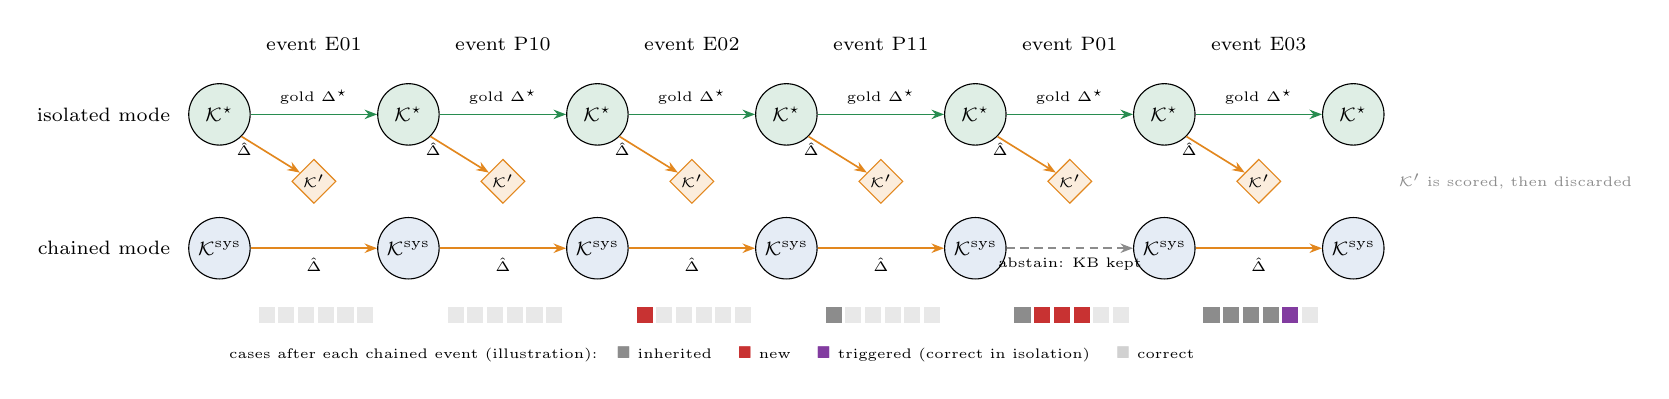
\begin{tikzpicture}[kb/.style={draw, circle, minimum size=0.78cm, font=\scriptsize, inner sep=0pt},
  sq/.style={minimum size=0.22cm, draw=white, line width=0.4pt, inner sep=0pt}]
\node[font=\scriptsize, anchor=east] at (-0.5,1.7) {isolated mode};
\node[font=\scriptsize, anchor=east] at (-0.5,0) {chained mode};
\foreach \lab [count=\i from 0] in {E01,P10,E02,P11,P01,E03}{
  \node[font=\scriptsize] at (\i*2.4+1.2,2.6) {event \lab};
  \node[kb, fill=chum!15] (g\i) at (\i*2.4,1.7) {$\mathcal{K}^\star$};
  \node[kb, fill=cdet!12] (c\i) at (\i*2.4,0) {$\mathcal{K}^{\mathrm{sys}}$};}
\node[kb, fill=chum!15] (g6) at (14.4,1.7) {$\mathcal{K}^\star$};
\node[kb, fill=cdet!12] (c6) at (14.4,0) {$\mathcal{K}^{\mathrm{sys}}$};
\foreach \i [evaluate=\i as \j using int(\i+1)] in {0,...,5}{
  \draw[ar, chum] (g\i) -- node[above, font=\tiny, text=black]{gold $\Delta^\star$} (g\j);
  \node[draw=cai, fill=cai!15, diamond, inner sep=0.8pt, font=\tiny] (k\i) at (\i*2.4+1.2,0.85) {$\mathcal{K}'$};
  \draw[ar, cai] (g\i.south east) -- node[left, font=\tiny, text=black, pos=0.35]{$\hat\Delta$} (k\i);}
\foreach \i [evaluate=\i as \j using int(\i+1)] in {0,1,2,3,5}{
  \draw[ar, cai] (c\i) -- node[below, font=\tiny, text=black]{$\hat\Delta$} (c\j);}
\draw[ar, cgr, densely dashed] (c4) -- node[below, font=\tiny, text=black]{abstain: KB kept} (c5);
\node[font=\tiny, text=cgr, anchor=west] at (14.85,0.85) {$\mathcal{K}'$ is scored, then discarded};
\foreach \i/\cols in {0/{cgr!20,cgr!20,cgr!20,cgr!20,cgr!20,cgr!20}, 1/{cgr!20,cgr!20,cgr!20,cgr!20,cgr!20,cgr!20},
  2/{cred,cgr!20,cgr!20,cgr!20,cgr!20,cgr!20}, 3/{cgr,cgr!20,cgr!20,cgr!20,cgr!20,cgr!20},
  4/{cgr,cred,cred,cred,cgr!20,cgr!20}, 5/{cgr,cgr,cgr,cgr,cpur,cgr!20}}{
  \foreach \c [count=\k from 0] in \cols {\node[sq, fill=\c] at (\i*2.4+0.6+\k*0.25,-0.85) {};}}
\node[font=\tiny, anchor=west] at (0,-1.35) {cases after each chained event (illustration):\quad
  \textcolor{cgr}{$\blacksquare$} inherited \quad \textcolor{cred}{$\blacksquare$} new \quad
  \textcolor{cpur}{$\blacksquare$} triggered (correct in isolation) \quad \textcolor{cgr!40}{$\blacksquare$} correct};
\end{tikzpicture}}}

% ------------------------------------------------------------------------------------------- architecture
\newcommand{\figArchitecture}{%
\resizebox{0.95\textwidth}{!}{%
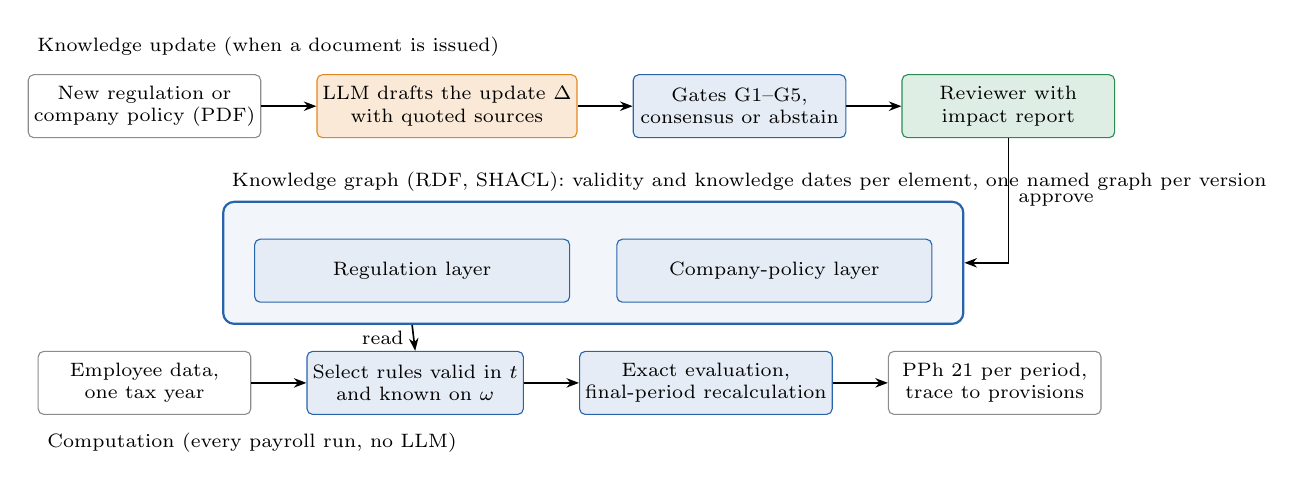
\begin{tikzpicture}[node distance=5mm and 7mm]
\node[bsrc, minimum width=2.7cm] (doc) {New regulation or\\company policy (PDF)};
\node[bai, right=of doc, minimum width=2.7cm] (llm) {LLM drafts the update $\Delta$\\with quoted sources};
\node[bdet, right=of llm, minimum width=2.7cm] (gate) {Gates G1--G5,\\consensus or abstain};
\node[bhum, right=of gate, minimum width=2.7cm] (rev) {Reviewer with\\impact report};
\draw[ar] (doc)--(llm); \draw[ar] (llm)--(gate); \draw[ar] (gate)--(rev);
\node[draw=cdet, fill=cdet!6, thick, rounded corners, minimum width=9.4cm, minimum height=1.55cm,
  below=12mm of $(llm)!0.5!(gate)$] (kb) {};
\node[bdet, minimum width=4cm] at ($(kb.center)+(-2.3,-0.1)$) {Regulation layer};
\node[bdet, minimum width=4cm] at ($(kb.center)+(2.3,-0.1)$) {Company-policy layer};
\node[font=\scriptsize, anchor=south west] at (kb.north west) {Knowledge graph (RDF, SHACL): validity and
  knowledge dates per element, one named graph per version};
\draw[ar] (rev.south) |- node[pos=0.25, right, font=\scriptsize]{approve} (kb.east);
\node[bsrc, below=27mm of doc, minimum width=2.7cm] (emp) {Employee data,\\one tax year};
\node[bdet, right=of emp, minimum width=2.7cm] (sel) {Select rules valid in $t$\\and known on $\omega$};
\node[bdet, right=of sel, minimum width=2.7cm] (calc) {Exact evaluation,\\final-period recalculation};
\node[bsrc, right=of calc, minimum width=2.7cm] (out) {PPh 21 per period,\\trace to provisions};
\draw[ar] (emp)--(sel); \draw[ar] (sel)--(calc); \draw[ar] (calc)--(out);
\draw[ar] ($(kb.south)+(-2.3,0)$) -- node[left, font=\scriptsize]{read} (sel.north);
\node[font=\scriptsize, anchor=west] at ($(doc.north west)+(0,0.35)$) {Knowledge update (when a document is issued)};
\node[font=\scriptsize, anchor=west] at ($(emp.south west)+(0,-0.35)$) {Computation (every payroll run, no LLM)};
\end{tikzpicture}}}

% ------------------------------------------------------------------------------------------- bitemporal
\newcommand{\figBitemporal}{%
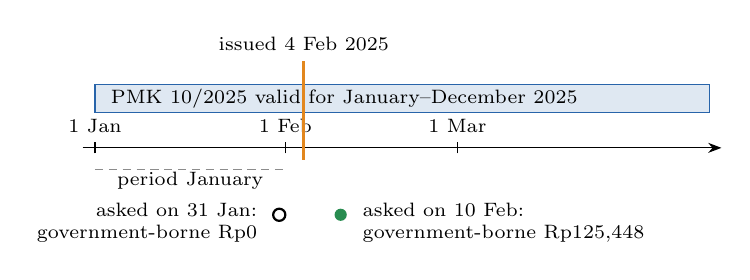
\begin{tikzpicture}[x=0.078cm]
\fill[cdet!15, draw=cdet] (0,1.05) rectangle (100,1.4);
\node[font=\scriptsize, anchor=west] at (1,1.225) {PMK 10/2025 valid for January--December 2025};
\draw[-{Stealth}] (-2,0.6) -- (102,0.6);
\foreach \x/\l in {0/1 Jan, 31/1 Feb, 59/1 Mar}{\draw (\x,0.53)--(\x,0.67) node[above, font=\scriptsize]{\l};}
\draw[cai, very thick] (34,0.45) -- (34,1.7) node[above, font=\scriptsize, text=black]{issued 4 Feb 2025};
\draw[densely dashed, cgr] (0,0.32) -- (31,0.32); \node[font=\scriptsize] at (15.5,0.18) {period January};
\fill[white, draw=black, thick] (30,-0.25) circle (2.2pt);
\node[font=\scriptsize, anchor=east, align=right] at (28,-0.35) {asked on 31 Jan:\\government-borne Rp0};
\fill[chum] (40,-0.25) circle (2.2pt);
\node[font=\scriptsize, anchor=west, align=left] at (42,-0.35) {asked on 10 Feb:\\government-borne Rp125,448};
\end{tikzpicture}}

% ------------------------------------------------------------------------------------------- engine
\newcommand{\figEngine}{%
\resizebox{0.98\textwidth}{!}{%
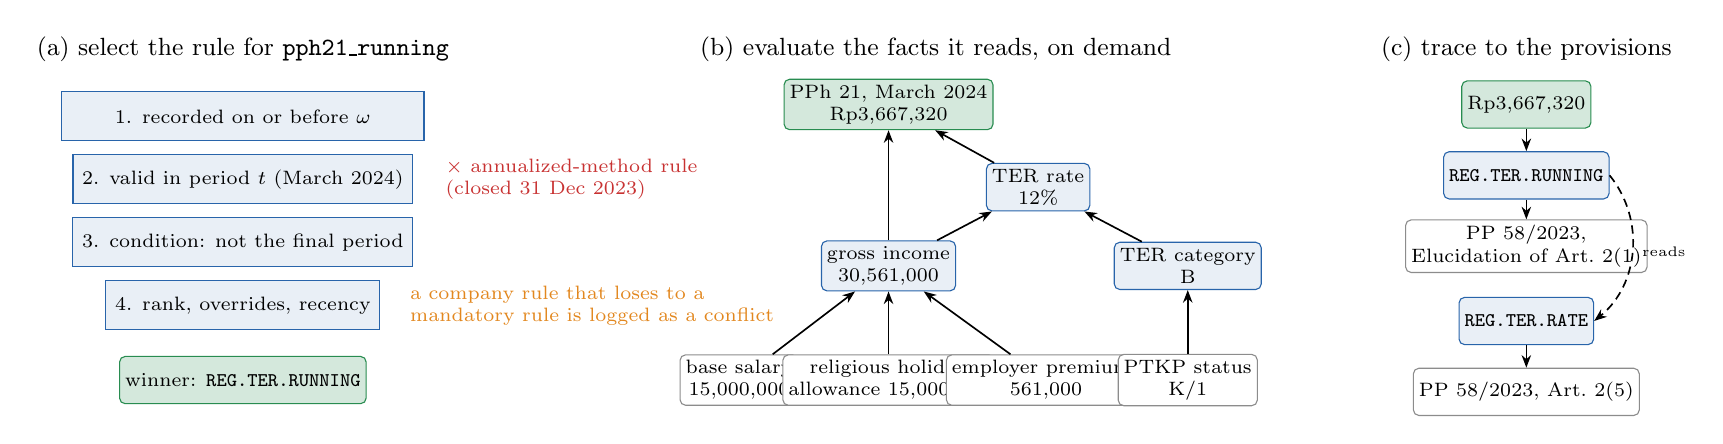
\begin{tikzpicture}[f/.style={draw=cdet, fill=cdet!10, rounded corners=2pt, font=\scriptsize, align=center,
  minimum height=0.6cm, inner sep=2pt}, inp/.style={f, fill=white, draw=cgr}]
\node[font=\small] at (2.3,4.75) {(a) select the rule for \texttt{pph21\_running}};
\foreach \y/\w/\t in {3.9/4.6/{1. recorded on or before $\omega$}, 3.1/4.0/{2. valid in period $t$ (March 2024)},
  2.3/3.4/{3. condition: not the final period}, 1.5/2.8/{4. rank, overrides, recency}}{
  \node[draw=cdet, fill=cdet!10, minimum width=\w cm, minimum height=0.62cm, font=\scriptsize] at (2.3,\y) {\t};}
\node[f, fill=chum!20, draw=chum] at (2.3,0.55) {winner: \texttt{REG.TER.RUNNING}};
\node[font=\scriptsize, text=cred, anchor=west, align=left] at (4.75,3.1) {$\times$ annualized-method rule\\(closed 31 Dec 2023)};
\node[font=\scriptsize, text=cai, anchor=west, align=left] at (4.3,1.5) {a company rule that loses to a\\mandatory rule is logged as a conflict};
\node[font=\small] at (11.1,4.75) {(b) evaluate the facts it reads, on demand};
\node[inp] (bs) at (8.6,0.55) {base salary\\15,000,000};
\node[inp] (thr) at (10.5,0.55) {religious holiday\\allowance 15,000,000};
\node[inp] (prem) at (12.5,0.55) {employer premiums\\561,000};
\node[inp] (st) at (14.3,0.55) {PTKP status\\K/1};
\node[f] (gross) at (10.5,2.0) {gross income\\30,561,000};
\node[f] (cat) at (14.3,2.0) {TER category\\B};
\node[f] (rate) at (12.4,3.0) {TER rate\\12\%};
\node[f, fill=chum!20, draw=chum] (pph) at (10.5,4.05) {PPh 21, March 2024\\Rp3,667,320};
\draw[ar] (bs)--(gross); \draw[ar] (thr)--(gross); \draw[ar] (prem)--(gross); \draw[ar] (st)--(cat);
\draw[ar] (gross)--(rate); \draw[ar] (cat)--(rate); \draw[ar] (rate)--(pph); \draw[ar] (gross)--(pph);
\node[font=\small] at (18.6,4.75) {(c) trace to the provisions};
\node[f, fill=chum!20, draw=chum] (t1) at (18.6,4.05) {Rp3,667,320};
\node[f] (t2) at (18.6,3.15) {\texttt{REG.TER.RUNNING}};
\node[inp] (t3) at (18.6,2.25) {PP 58/2023,\\Elucidation of Art.~2(1)};
\node[f] (t4) at (18.6,1.3) {\texttt{REG.TER.RATE}};
\node[inp] (t5) at (18.6,0.4) {PP 58/2023, Art.~2(5)};
\draw[ar] (t1)--(t2); \draw[ar] (t2)--(t3); \draw[ar, densely dashed] (t2.east) to[bend left=45]
  node[right, font=\tiny]{reads} (t4.east); \draw[ar] (t4)--(t5);
\end{tikzpicture}}}

% ------------------------------------------------------------------------------------------- acquisition flow
\newcommand{\figAcquisitionFlow}{%
\resizebox{0.95\textwidth}{!}{%
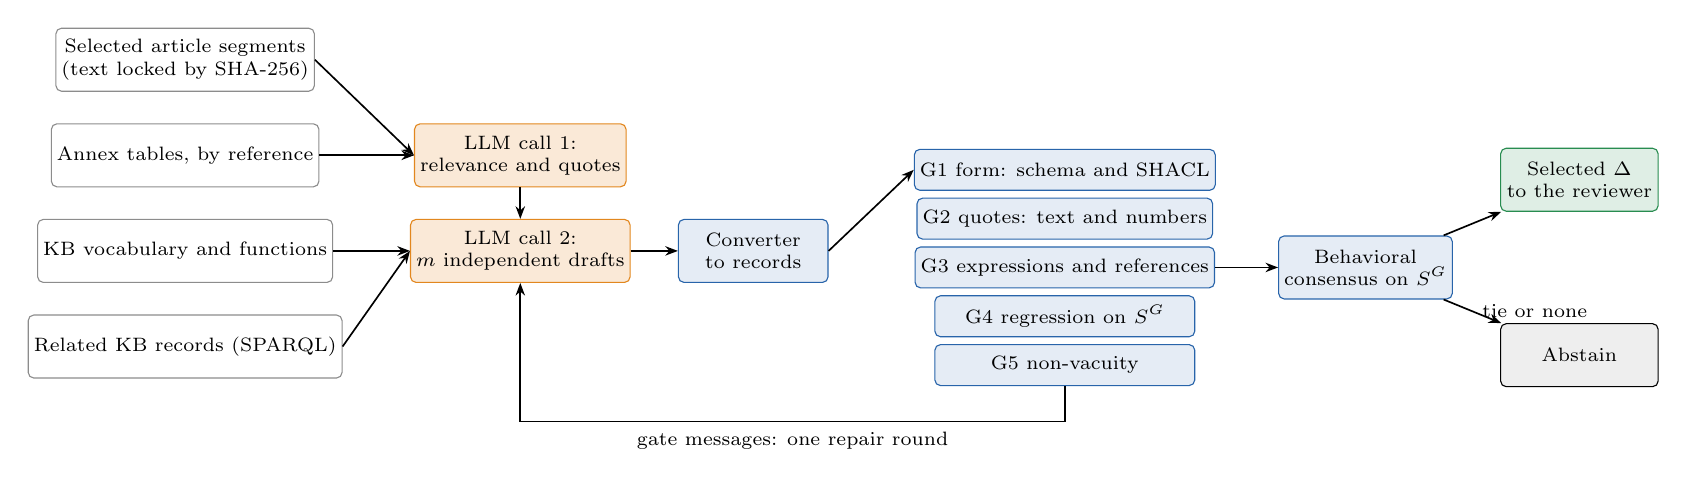
\begin{tikzpicture}[node distance=4mm and 6mm]
\node[bsrc, minimum width=3cm] (seg) {Selected article segments\\(text locked by SHA-256)};
\node[bsrc, below=of seg, minimum width=3cm] (tab) {Annex tables, by reference};
\node[bsrc, below=of tab, minimum width=3cm] (voc) {KB vocabulary and functions};
\node[bsrc, below=of voc, minimum width=3cm] (rec) {Related KB records (SPARQL)};
\node[bai, right=12mm of tab, minimum width=2.5cm] (rel) {LLM call 1:\\relevance and quotes};
\node[bai, below=of rel, minimum width=2.5cm] (dr) {LLM call 2:\\$m$ independent drafts};
\node[bdet, right=of dr, minimum width=1.9cm] (conv) {Converter\\to records};
\foreach \g/\n [count=\i] in {G1/form: schema and SHACL,G2/quotes: text and numbers,G3/expressions and references,
  G4/regression on $S^G$,G5/non-vacuity}{
  \node[bdet, minimum width=3.3cm, minimum height=0.52cm] (g\i) at ($(conv.east)+(3.0,1.65-\i*0.62)$) {\g\ \n};}
\node[bdet, right=8mm of g3, minimum width=2.2cm] (cons) {Behavioral\\consensus on $S^G$};
\node[bhum, above right=3mm and 6mm of cons, minimum width=2cm] (sel) {Selected $\Delta$\\to the reviewer};
\node[b, below right=3mm and 6mm of cons, minimum width=2cm, fill=cgr!15] (abs) {Abstain};
\draw[ar] (seg.east) -- (rel.west); \draw[ar] (tab.east)--(rel.west); \draw[ar] (voc.east)--(dr.west);
\draw[ar] (rec.east)--(dr.west);
\draw[ar] (rel)--(dr); \draw[ar] (dr)--(conv); \draw[ar] (conv.east)--(g1.west);
\draw[ar] (g5.south) -- ++(0,-0.45) -| node[pos=0.25, below, font=\scriptsize]{gate messages: one repair round} (dr.south);
\draw[ar] (g3.east)--(cons); \draw[ar] (cons)--(sel); \draw[ar] (cons)--node[right, font=\scriptsize]{tie or none} (abs);
\end{tikzpicture}}}

% ------------------------------------------------------------------------------------------- case study
\newcommand{\figCaseStudy}{%
\resizebox{0.97\textwidth}{!}{%
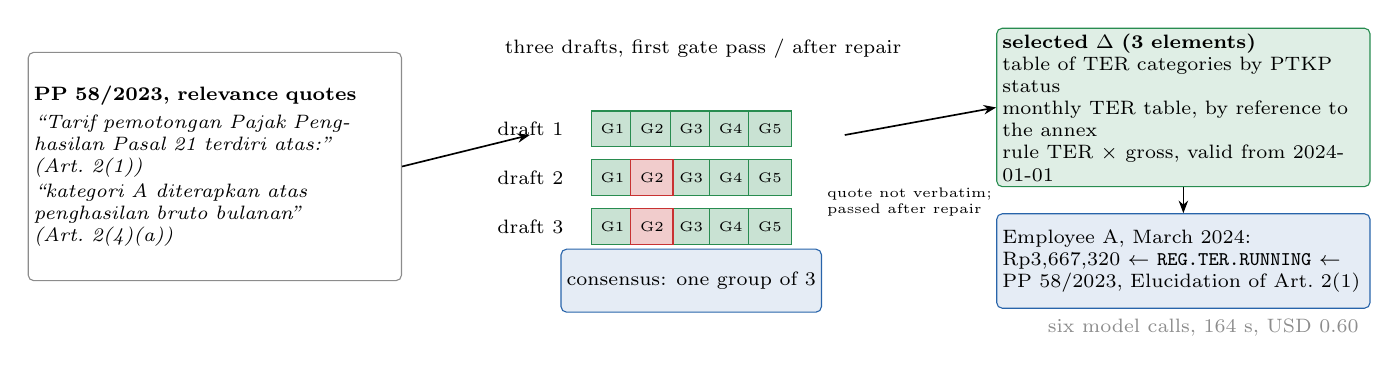
\begin{tikzpicture}
\node[bsrc, text width=4.6cm, align=left, minimum height=2.9cm] (q) at (0,0) {\textbf{PP 58/2023, relevance quotes}\\[2pt]
  \itshape ``Tarif pemotongan Pajak Penghasilan Pasal 21 terdiri atas:'' (Art.~2(1))\\[1pt]
  ``kategori A diterapkan atas penghasilan bruto bulanan'' (Art.~2(4)(a))};
\node[font=\scriptsize] at (6.2,1.5) {three drafts, first gate pass / after repair};
\foreach \d/\st [count=\i] in {1/{pass,pass,pass,pass,pass},2/{pass,fail,,,},3/{pass,fail,,,}}{
  \node[font=\scriptsize, anchor=east] at (4.55,1.1-\i*0.62) {draft \d};
  \foreach \g [count=\j] in {G1,G2,G3,G4,G5}{
    \node[draw=chum, fill=chum!25, font=\tiny, minimum size=0.45cm] at (4.55+\j*0.5,1.1-\i*0.62) {\g};}}
\node[draw=cred, fill=cred!25, font=\tiny, minimum size=0.45cm] at (5.55,-0.14) {G2};
\node[draw=cred, fill=cred!25, font=\tiny, minimum size=0.45cm] at (5.55,-0.76) {G2};
\node[font=\tiny, anchor=west, align=left] at (7.65,-0.45) {quote not verbatim;\\passed after repair};
\node[bdet, font=\scriptsize] at (6.05,-1.45) {consensus: one group of 3};
\node[bhum, text width=4.6cm, align=left, minimum height=1.5cm, font=\scriptsize] (d) at (12.3,0.75) {\textbf{selected $\Delta$ (3 elements)}\\
  table of TER categories by PTKP status\\monthly TER table, by reference to the annex\\rule TER $\times$ gross, valid from 2024-01-01};
\node[bdet, text width=4.6cm, align=left, minimum height=1.2cm, font=\scriptsize] (t) at (12.3,-1.2) {Employee A, March 2024:\\
  Rp3,667,320 $\leftarrow$ \texttt{REG.TER.RUNNING} $\leftarrow$\\PP 58/2023, Elucidation of Art.~2(1)};
\draw[ar] (q.east)--(4.0,0.4); \draw[ar] (8.0,0.4)--(d.west); \draw[ar] (d)--(t);
\node[font=\scriptsize, text=cgr, anchor=east] at (14.65,-2.05) {six model calls, 164 s, USD 0.60};
\end{tikzpicture}}}


\begin{document}
\bstctlcite{IEEEexample:BSTcontrol}
\history{Date of publication xxxx 00, 0000, date of current version xxxx 00, 0000.}
\doi{10.1109/ACCESS.2026.DOI}

\title{An Adaptive Knowledge-Based System for PPh 21 Calculation with LLM-Assisted Knowledge Acquisition from Regulations and Company Policies}

\author{\uppercase{Obi Kastanya}\authorrefmark{1}
AND \uppercase{Mahathir Muhammad}\authorrefmark{1}}

\address[1]{Department of Informatics, Institut Teknologi Sepuluh Nopember, Surabaya 60111, Indonesia
(e-mail: 6025252015@student.its.ac.id; 6025252008@student.its.ac.id)}
\tfootnote{This work received no external funding.}

\markboth
{Kastanya and Muhammad: Adaptive Knowledge-Based System for PPh 21 Calculation}
{Kastanya and Muhammad: Adaptive Knowledge-Based System for PPh 21 Calculation}

\corresp{Corresponding author: Obi Kastanya (e-mail: 6025252015@student.its.ac.id).}

\begin{abstract}
Indonesian employers withhold Income Tax Article 21 monthly under rules that changed 13 times between 2023 and 2026, five of them retroactively, while most payroll calculators hard-code them. This paper presents an adaptive knowledge-based system in which regulations and company policies form a two-layer knowledge graph that records when each rule is valid and when it became known. A deterministic engine computes the tax with a trace to the legal provisions, and a large language model only drafts updates from new documents. Each draft must quote its source, pass five automatic checks, and compete with independent drafts in a behavioral vote, and it enters the knowledge base only after a reviewer approves it. The evaluation replayed the 13 real changes and 20 distractor documents against 2,398 employee-year test cases, scored five collective labor agreements on separate cases, and added 16 changes unseen by the designers. The representation expressed all 16 unseen changes without modifying the engine once the rounding convention of their examples was aligned. Drafted updates were correct for 8 of 18 real documents and silently wrong for 3, and each silent error changed withholding by more than Rp1,000 for at least two employees. All five single-element updates succeeded, whereas none of the nine documents that needed 11 or more elements did, including the five labor agreements. Language models can thus draft parameter updates for an executable tax knowledge base, while structural regulations and company policies still need a reviewer supported by the system's impact reports.
\end{abstract}

\begin{keywords}
Knowledge acquisition, knowledge-based systems, large language models, regulatory change, tax computation.
\end{keywords}

\titlepgskip=-21pt

\maketitle

% ============================================================================
\section{Introduction}
\label{sec:intro}
% ============================================================================
\PARstart{I}{ndonesian} employers withhold Income Tax Article 21 (PPh 21) from the pay of every employee each month, so an error in the rules reaches every payslip and every withholding slip. The rules change often. Between 2023 and 2026, 13 regulatory events changed the PPh 21 computation for permanent employees, and seven of them were issued in 2025 (Fig.~\ref{fig:timeline}). Government Regulation (PP) 58/2023 and its implementing Minister of Finance Regulation (PMK) 168/2023 replaced the annualized monthly method with average effective rates (TER) from January 2024. Both were issued in the last week of December 2023~\cite{pp58_2023,pmk168_2023}. Five events took effect retroactively. PMK 10/2025 made the government bear the tax of certain employees (DTP). It was issued on 4 February 2025 but covers January 2025, so a January payroll that was correct when it ran became wrong a month later~\cite{pmk10_2025}.

\begin{figure*}[!t]
\centering
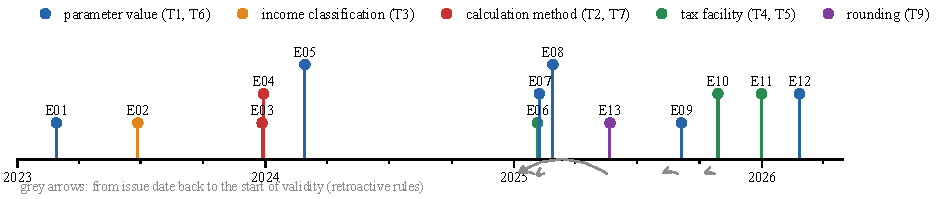
\includegraphics[width=\textwidth]{figs/fig_timeline.pdf}
\caption{Regulatory events that changed PPh 21 for permanent employees, 2023--2026, at their issue dates. Colors group the change types of Table~\ref{tab:types}; grey arrows run from the issue date back to the start of validity for the five retroactive rules.}
\label{fig:timeline}
\end{figure*}

Payroll software usually encodes these rules in program code or spreadsheets~\cite{ramadhani2021grossup,kusuma2026pph21}, so every regulation needs new code. Two open-source PPh 21 calculators added TER 26 and 915 days after PP 58/2023 was issued and changed 163 and 504 lines of code (Section~\ref{sec:res-compare}). Nothing in either change shows that earlier periods keep their results, and a company policy that the new rule makes noncompliant goes unnoticed. A knowledge-based system (KBS) separates the rules from the code that executes them~\cite{merigoux2021catala}, but the burden moves to keeping the knowledge base (KB) current. Large language models (LLMs) can turn legal text into structured rules~\cite{janatian2023texttostructure}, yet they are unreliable when asked to compute tax directly~\cite{nay2024taxattorneys,dahl2024legalfictions}.

Work that combines LLMs with tax rules builds a rule base for the law at one point in time. The closest exception updated a tax program by one legal year with LLM-written candidates selected by majority vote~\cite{goganikhiabani2025maintaining}, without testing earlier periods or a chain of updates. Earlier work has not measured whether repeated LLM-drafted updates of an executable legal rule base keep the results of earlier periods, or whether an error in one update spreads to later ones. It has also not measured how such an update affects the policies that companies layer on top of the regulation (Table~\ref{tab:position} in Section~\ref{sec:related}).

This paper addresses those questions with a KBS for PPh 21 whose knowledge is a two-layer knowledge graph, with one layer for regulations and one for company policies (Fig.~\ref{fig:architecture}). Every element of the graph records both its legal validity and the date it became known. A deterministic engine computes the tax and traces each value to the provisions it rests on. An LLM only drafts knowledge updates. Each draft must quote the document, passes five verification gates, and competes with independent drafts in a behavioral consensus that abstains when the drafts disagree; a reviewer approves the result. The study measures four properties of this design: the expressiveness of the representation, the safety of a single LLM-drafted update, the stability of updates applied in chronological order, and the detection of company policies affected by a regulatory change.

The contributions are:
\begin{enumerate}
\item A bitemporal two-layer representation of PPh 21 as an RDF knowledge graph with executable rules, conflict resolution between the layers, and a trace to the provisions (Section~\ref{sec:system}). It expressed 16 changes unseen by its designers without engine modifications once the rounding convention of their examples was aligned.
\item An incremental acquisition pipeline in which an LLM drafts updates with quoted sources, deterministic gates and behavioral consensus filter them, and a reviewer receives an impact report (Section~\ref{sec:system}). Ablations attribute its gain over a single draft to consensus and abstention, not to the gates.
\item A regulation-replay protocol that applies real changes in chronological order, in isolation and in a chain, and separates inherited, new, and triggered errors (Sections~\ref{sec:formulation} and~\ref{sec:design}).
\item An evaluation on the 13 regulatory events of 2023--2026 and five collective labor agreements that shows for which kinds of change an LLM-drafted update can be trusted (Section~\ref{sec:results}). The knowledge base, corpus, test cases, and logs are released.
\end{enumerate}
Section~\ref{sec:background} summarizes PPh 21 for readers outside Indonesia, Section~\ref{sec:related} positions the work, Sections~\ref{sec:formulation}--\ref{sec:casestudy} define the problem and the system, Sections~\ref{sec:design}--\ref{sec:results} report the evaluation, and Sections~\ref{sec:discussion} and~\ref{sec:conclusion} discuss and conclude.

% ============================================================================
\section{Background: Payroll Income Tax in Indonesia}
\label{sec:background}
% ============================================================================
The rest of the paper relies on three parts of PPh 21: how the monthly tax is computed, how its rules change, and how far a company may set its own payroll rules.

\subsection{Computing PPh 21 for a Permanent Employee}
\label{sec:pph21}
The monthly gross income of a permanent employee includes the salary, fixed allowances, and irregular payments such as the religious holiday allowance (THR) and bonuses. It also includes the work-accident, death, and health premiums that the employer pays and, since July 2023, benefits in kind. Until 2023 the employer annualized each month's regular income and deducted the occupational expense, the employee's pension contributions, and the nontaxable amount (PTKP) of the employee's family status. The result was taxed at the five progressive rates of Article 17, from 5\% to 35\%~\cite{uu7_2021,pmk101_2016,per16_2016}. Since January 2024 the months from January to November apply a monthly effective rate (TER) to gross income. The rate depends on the gross amount and on a category, A, B, or C, that follows from the PTKP status. The final period recomputes the tax of the whole year under Article 17 and withholds the difference from what was already withheld~\cite{pp58_2023,pmk168_2023}.

The running example of this paper is Employee A, with status K/1 (married, one dependent, category B), a monthly salary of Rp15,000,000, and a THR of the same amount paid in March. Table~\ref{tab:slip} applies both methods to this employee. TER raises the March withholding to 12\% of a gross of Rp30,561,000, and the December recalculation then withholds only Rp186,480 because the earlier months already covered most of the annual tax. The annual totals differ by Rp8,700, but the monthly profiles do not. The regular withholding of 2023 is Rp725 lower from April onward because the pension wage cap rose in March (event E01 in Fig.~\ref{fig:timeline}), which raised the deductible pension contribution.

\begin{table}[!t]
\caption{Running example: monthly PPh 21 of Employee A (K/1, salary Rp15,000,000, THR in March) under the annualized method of 2023 and the TER method of 2024, as computed by the engine from the gold knowledge base.}
\label{tab:slip}
\centering\footnotesize
\setlength{\tabcolsep}{4pt}
\begin{tabular}{@{}lrrrr@{}}
\toprule
Period & Gross (Rp) & 2023 (Rp) & TER 2024 & 2024 (Rp) \\
\midrule
January, February & 15,561,000 & 913,025 & B, 6\% & 933,660 \\
March (THR) & 30,561,000 & 3,162,300 & B, 12\% & 3,667,320 \\
April--November & 15,561,000 & 912,300 & B, 6\% & 933,660 \\
December & 15,561,000 & 912,350 & Article 17 & 186,480 \\
\midrule
Year & 201,732,000 & 13,199,100 & & 13,190,400 \\
\bottomrule
\end{tabular}
\end{table}

\subsection{How the Rules Change}
\label{sec:changes}
Ten types of change, fixed before any model output existed, structure the corpus and the reporting of results (Table~\ref{tab:types}). Two dates matter for every change. The issue date is when the rule becomes known, and the start of validity is when it binds. The two dates coincide for most parameter letters. A retroactive rule separates them and makes the correct value of a past period depend on the date on which the question is asked. An example is the rounding rule of Director General Regulation PER-11/PJ/2025, issued in May 2025 for periods from January 2025. A KB that records only validity cannot reproduce what an employer should have withheld with the knowledge available at the time, which is why the representation of Section~\ref{sec:system} records both dates.

\begin{table}[!t]
\caption{Types of regulatory change, with the events of the test corpus that belong to each type.}
\label{tab:types}
\centering\footnotesize
\setlength{\tabcolsep}{3pt}
\begin{tabularx}{\columnwidth}{@{}lLl@{}}
\toprule
Code & Type of change & Test events \\
\midrule
T1 & a single parameter value (wage cap, rate, ceiling) & E01, E05, E07, E08, E12 \\
T2 & a rate table is created or changed & E03 \\
T3 & income classification & E02, E04 \\
T4 & a new facility with eligibility criteria & E06, E11 \\
T5 & the scope of a facility & E10 \\
T6 & the validity period of a rule & E09 \\
T7 & a change of calculation method & E03, E04 \\
T8 & repeal without replacement & none \\
T9 & a calculation procedure such as rounding & E13 \\
T10 & a company policy & labor agreements \\
\bottomrule
\end{tabularx}
\end{table}

\subsection{Company Policies and Their Legal Limits}
\label{sec:policies}
Employers decide parts of the payroll themselves through company regulations or collective labor agreements (PKB): proration for partial months, the THR formula, and whether the employer bears the tax. These policies may not override mandatory provisions. Article 22(3) of the 2025--2026 agreement of PT Wijaya Karya states that government tax incentives are not passed on to employees. PMK 10/2025, in contrast, requires in Article 5(1) that the employer pay the government-borne tax to the employee in cash~\cite{pmk10_2025}. The conflict stays latent because the company is not in an eligible sector; a regulatory change that widened the sectors would activate it. Ten conflict types, from a misclassified income component to a missed minimum entitlement, are listed in Appendix~\ref{app:taxonomies}.

\subsection{Scope and Assumptions}
The study covers permanent employees of private and state-owned employers, one employee per computation, and tax years 2023--2026, with regulatory history from 2012 used for development. It excludes non-permanent workers, severance and other income taxed at final rates, the higher rate for employees without a tax identification number, batch payroll runs, and the filing of withholding slips. Every employee is assumed to hold a valid tax identification, and payroll inputs are taken as recorded.

% ============================================================================
\section{Related Work}
\label{sec:related}
% ============================================================================
Five lines of work meet in this study: rules-as-code systems, incremental knowledge acquisition, LLM-based formalization of law, the evaluation of repeated LLM updates, and temporal legal knowledge graphs. The search for the closest work covered publications up to November 2026 and relied mostly on titles and abstracts; papers of ICAIL 2026 were available only through arXiv.

\subsection{Rules as Code and Payroll Tax Systems}
Catala translates statutes into a programming language with general cases and exceptions based on default logic, and its evaluation found bugs in an official implementation~\cite{merigoux2021catala,huttner2022catala}. Mlang replaced the legacy compiler of the French income-tax engine~\cite{merigoux2021mlang}, and the same ecosystem formalizes date arithmetic~\cite{monat2024date} and generates test cases by concolic execution~\cite{goutagny2025cutecat}. DataLex~\cite{mowbray2023scaling,mowbray2023xai} and Logical English~\cite{kowalski2022logicalenglish} follow the same principle. Meessen shows that many normative decisions end up inside technical components~\cite{meessen2023arrows}, and Witt et al.\ separate technical validation from legal conformity~\cite{witt2024encoding}. Dumancic et al.\ state payroll tax and social-security legislation declaratively for policy optimization~\cite{dumancic2021payroll}, and Al-Hawari et al.\ build a rule-based payroll system~\cite{alhawari2026payroll}. Indonesian PPh 21 systems are mostly procedural~\cite{ramadhani2021grossup,yulistyawati2022payroll,kusuma2026pph21}, and TER produces overwithholding on irregular income~\cite{sherra2025ter}. People write the knowledge in all of these systems, and none of them evaluates updates written by a machine.

\subsection{Incremental Knowledge Acquisition}
Ripple-Down Rules add a rule whenever an expert finds a wrong case, and cornerstone cases keep the new rule from breaking cases that were already right~\cite{compton2021rdr}. The regression gate G4 of this study plays the role of the cornerstone cases. Work on legal logic formalizes changes of law and theory revision with temporalized revision operators~\cite{moguillansky2024temporalised}, and shows that revising defeasible theories is computationally hard~\cite{olivieri2025revising}. Other work shows how unexpected consequences can be traced back to the rules that cause them~\cite{fungwacharakorn2021debugging}. An expert still writes every change in this line of work.

\subsection{LLMs for Legal and Tax Formalization}
LLMs have turned legal text into structures for legal expert systems~\cite{janatian2023texttostructure}, drafted Decision Model and Notation rules for an accounting office~\cite{makowski2025dmn}, and derived metamorphic relations for testing tax software~\cite{srinivas2023fewshot,khiabani2026agentic}. Veeramani et al.\ store the Indian Income Tax Act as a knowledge graph executed by a symbolic rule engine, with an LLM extracting the graph, and reach 80\% accuracy on 20 scenarios~\cite{veeramani2026neurosymbolic}. Yadamsuren et al.\ formalize one section of the United States Internal Revenue Code in Prolog to detect a known inconsistency~\cite{yadamsuren2026formalization}. Lorenzo et al.\ benchmark the translation of French tax provisions into Catala by code similarity and syntactic validity, without executing the output~\cite{lorenzo2025translating}. Jurayj et al.\ combine an LLM with a Prolog solver on 100 tax cases, where o3 gives 75 correct answers, 15 wrong answers, and 10 abstentions without gold statutes~\cite{jurayj2026tax}. LLM performance on tax law improves across model generations without reaching expert level~\cite{blairstanek2023gpt3,nay2024taxattorneys}, and commercial legal research tools still hallucinate~\cite{magesh2025hallucination}.

These systems formalize the law as it stands at one time. The nearest exception is the work of Gogani-Khiabani et al., who ask an LLM to update United States tax code from 2020 to 2021 and select candidates by behavioral majority vote~\cite{goganikhiabani2025maintaining}. Their accuracy with the previous year's code as context ranges from 21\% to 100\% for GPT-3.5 and from 48\% to 100\% for GPT-4.0. Their study covers one step, does not test earlier periods, and does not measure error propagation. The consensus of the present system uses the same selection idea and adds verification gates and abstention.

\subsection{Repeated LLM Updates and Their Evaluation}
Sequential knowledge editing degrades a language model after many edits~\cite{gupta2024editing,gu2024harms}. KoLEG keeps performance above 95\% after four cumulative edits from Korean legal amendments~\cite{seo2025koleg}, but it edits the model and not a rule base. The same holds for updating model knowledge of changed code APIs~\cite{wu2026recode}. Prior et al.\ consolidate four German statutes with an LLM, and exact match falls from 50.3\% for a single amendment to 20.51\% for amendment chains~\cite{prior2025risks}. The object there is XML text rather than executed rules, and only the final version of each chain is compared. Execution-based measures such as pass@k~\cite{chen2021evaluating} and n@k~\cite{li2022alphacode} come from code generation, and selective prediction scores a model that may abstain by its risk and coverage~\cite{xin2021abstention}. These measures have not been applied to an executable, time-versioned legal rule base, and the metrics of Section~\ref{sec:design} build on them.

\subsection{Temporal Legal Knowledge Representation}
De Martim models norms as works with versioned expressions so that answers are not anachronistic~\cite{demartim2025satgraph}, and Kharraz et al.\ define conflicts in a temporal normative logic~\cite{kharraz2024conflicts}. The European Legislation Identifier (ELI)~\cite{publicationsoffice2026elien}, OWL-Time~\cite{cox2017owltime}, PROV-O~\cite{lebo2013provo}, and LegalRuleML~\cite{palmirani2021legalruleml} provide vocabularies for documents, time, provenance, and norms. The Shapes Constraint Language (SHACL)~\cite{knublauch2017shacl} provides validation, and this study reuses all of them except LegalRuleML. Norm-conflict detection~\cite{robaldo2024compliance,khoja2026consistency}, rule-base anomaly checking~\cite{boujelben2025anomalies}, testing of tax software when no reference outputs exist~\cite{tizpaz2023metamorphic,li2025mrgeneration}, property-based testing~\cite{goldstein2024pbt,ravi2025pbtpython}, and mutation analysis~\cite{petrovic2022mutation,petrovic2021mutation} inform the ground truth and test design of Section~\ref{sec:design}. Work in this group versions norms but does not evaluate machine-written updates of executed rules.

\subsection{Positioning}
Table~\ref{tab:position} compares the closest work on the three aspects that this study measures. No work in the table applies machine-drafted updates to an executable rule base repeatedly, measures how errors spread across those updates, and checks their effect on a company-policy layer. Gogani-Khiabani et al.\ come closest on the first aspect, with a single update step.

\begin{table*}[!t]
\caption{Position relative to the closest work. ``--'' means that the aspect is not reported as a focus of the cited publication.}
\label{tab:position}
\centering\footnotesize
\setlength{\tabcolsep}{3pt}
\begin{tabularx}{\textwidth}{@{}P{3.0cm} P{1.9cm} L P{2.0cm} P{1.6cm} P{1.5cm} P{1.2cm} P{2.3cm}@{}}
\toprule
Work & Domain & Representation & Knowledge author & Incremental update & Error spread measured & Company layer & Evaluation \\
\midrule
Catala~\cite{merigoux2021catala,huttner2022catala} & tax and benefits & domain-specific language, default logic & people & -- & -- & -- & bugs found in an official implementation \\
DataLex~\cite{mowbray2023scaling,mowbray2023xai} & legislation & semi-natural rule language and inference engine & people & -- & -- & -- & -- \\
Dumancic et al.~\cite{dumancic2021payroll} & payroll & formal model compiled to constraints & people & -- & -- & -- & use at a social-security agency \\
Ripple-Down Rules~\cite{compton2021rdr} & general & rules with exceptions & expert & yes & -- & -- & cornerstone cases \\
Veeramani et al.~\cite{veeramani2026neurosymbolic} & Indian income tax & knowledge graph and symbolic rules & LLM (graph), expert (rules) & proposed & -- & -- & 20 scenarios, 80\% \\
Yadamsuren et al.~\cite{yadamsuren2026formalization} & one section of US tax code & Prolog & LLM guided by people & -- & -- & -- & one known inconsistency \\
Lorenzo et al.~\cite{lorenzo2025translating} & French tax & Catala & LLM per provision & -- & -- & -- & 89 test samples, not executed \\
Jurayj et al.~\cite{jurayj2026tax} & US tax & Prolog & LLM per case & -- & -- & -- & 100 cases with abstention \\
Gogani-Khiabani et al.~\cite{goganikhiabani2025maintaining} & US tax & Python code & LLM & one step (2020 to 2021) & -- & -- & accuracy per scenario \\
Prior et al.~\cite{prior2025risks} & German statutes & XML text, not executed & LLM & yes, text & final version of chains & -- & 908 comparisons \\
PPh 21 systems~\cite{ramadhani2021grossup,yulistyawati2022payroll,kusuma2026pph21} & PPh 21 & procedural code or spreadsheets & people & -- & -- & -- & -- \\
\midrule
This study & PPh 21 & bitemporal two-layer knowledge graph with executable rules & LLM, gates, reviewer & yes & yes & yes & chronological regulation replay \\
\bottomrule
\end{tabularx}
\end{table*}

% ============================================================================
\section{Problem Formulation}
\label{sec:formulation}
% ============================================================================
A claim that a system ``adapts'' to a regulation is testable only when the expected behavior is defined case by case. This section defines the knowledge base, the result it computes, the conditions an update must satisfy, and the errors that a chain of updates can produce.

\subsection{Knowledge Base and Computation Result}
\begin{definition}[Knowledge base]
\label{def:kb}
A knowledge base $\K$ holds rule records, versioned parameters, table versions, mandatory constraints, and source documents. A rule $r = \langle \mathit{id}, \ell, \sigma, [t_s, t_e], t_c, \varphi, f \mathrel{:=} e, \mathit{ov}, \mathit{src} \rangle$ has a layer $\ell \in \{\text{regulation}, \text{company}\}$ and a modality $\sigma \in \{\text{mandatory}, \text{default}, \text{optional}\}$. It also has a validity period $[t_s, t_e]$ and a recording date $t_c$ equal to the issue date of its document. A condition $\varphi$, a fact $f$ with its expression $e$, the rules $\mathit{ov}$ it overrides, and quotes $\mathit{src}$ from its source complete the record. Records are never edited in place; a change adds a new version.
\end{definition}

\begin{definition}[Computation result]
\label{def:result}
$\result(\K, x, t, \omega)$ is the value of an output fact for case $x$ in tax period $t$, computed with the regulations known on date $\omega$ and the company policy of the case. A case is one employee at one employer for one tax year.
\end{definition}

The withholding of Employee A for March 2024 as known on 1 April 2024 is one such result. The gold knowledge base $\K^\gold$ is the reference that the authors built from the regulation texts and validated against external calculations (Section~\ref{sec:groundtruth}). The evaluation judges every update by comparing its results with those of $\K^\gold$.

\subsection{Updates and Adaptivity Conditions}
An update $\Delta$ for an event with issue date $t_{\mathit{iss}}$ and effective date $t_{\mathit{eff}}$ adds, changes, or removes elements, and $\K' = \K \oplus \Delta$. Gold updates satisfy $\K^{\gold}_n = \K^{\gold}_{n-1} \oplus \Delta^{\gold}_n$, and the correct update for a distractor document is empty.

\begin{definition}[Adaptivity conditions]
\label{def:conditions}
For a set of cases $S$: (A1) the engine code does not change; (A2) $\result(\K', x, t, \omega) = \result(\K^{\gold}, x, t, \omega)$ for every $x \in S$, $t \geq t_{\mathit{eff}}$, and $\omega \geq t_{\mathit{iss}}$; (A3$_t$) results for periods $t < t_{\mathit{eff}}$ do not change; (A3$_\omega$) results for knowledge dates $\omega < t_{\mathit{iss}}$ do not change; (A4) the conflict report of $\K'$ equals that of $\K^{\gold}$.
\end{definition}

Condition A3$_t$ means that adding the TER rules of 2024 must leave the December 2023 withholding of Employee A unchanged. Condition A3$_\omega$ means that an answer given before a regulation was issued must stay the answer the system would have given then. A1 and A3$_\omega$ hold by construction and are checked as invariants; A2, A3$_t$, and A4 are tested.

\subsection{Representational and Operational Adaptivity}
\begin{definition}[Adaptivity]
\label{def:adapt}
A representation is adaptive to an event if \emph{some} update $\Delta$ satisfies A1--A4. A system is operationally adaptive to an event if the update $\hat{\Delta}$ \emph{selected by its pipeline} satisfies A2, A3$_t$, and A4 on every case of the test space $\SE$, so that one wrong value makes $\hat{\Delta}$ wrong.
\end{definition}

The first definition concerns what the knowledge base can express; the second concerns what the LLM-assisted pipeline actually produces. Sections~\ref{sec:res-expressiveness} and~\ref{sec:res-single} test them separately.

\subsection{Error Types in a Chain of Updates}
\label{sec:errortypes}
An update can be applied in two modes (Fig.~\ref{fig:protocol}). Isolated mode applies the draft for event $n$ to the gold knowledge base before that event, $\K^\gold_{n-1}$, and scores and discards the result. Chained mode applies the draft to the system's own knowledge base $\K^{\mathrm{sys}}_{n-1}$, which already carries every earlier draft and every earlier abstention. A case that is wrong after event $n$ in chained mode falls into one of three groups. An inherited error was already wrong before event $n$, and a new error appears at event $n$. A triggered error is a new error on a case that is correct after the same event in isolated mode, so it exists only because of the chain.

\begin{figure*}[!t]
\centering
\figReplayProtocol
\caption{Regulation replay in isolated and chained mode. In isolated mode the gold knowledge base advances by the gold update and each draft $\hat{\Delta}$ is scored on a copy $\K'$; in chained mode each draft is applied to the system's own knowledge base, and an abstention leaves it unchanged. The squares illustrate how wrong cases are classified as inherited, new, or triggered.}
\label{fig:protocol}
\end{figure*}

% ============================================================================
\section{Proposed System}
\label{sec:system}
% ============================================================================
The system separates two paths that meet in the knowledge base (Fig.~\ref{fig:architecture}). A language model takes part only in the knowledge-update path, which runs when a regulation or company policy is issued. The computation path runs at every payroll calculation and is deterministic.

\begin{figure*}[!t]
\centering
\figArchitecture
\caption{System architecture. The language model only drafts knowledge updates on the upper path; a reviewer approves them into the two-layer knowledge graph, and every computation on the lower path is deterministic and traced to legal provisions. Orange marks the language model, blue deterministic code, and green the human decision.}
\label{fig:architecture}
\end{figure*}

\subsection{Knowledge Representation}
\label{sec:representation}
GraphDB stores the structural knowledge as an RDF and OWL knowledge graph with SHACL validation and SPARQL queries (Fig.~\ref{fig:ontology}). The graph holds documents, provisions, quotes, rules, parameters, tables, company policies, change events, updates, and knowledge-base versions. The ontology reuses ELI for legal documents and provisions~\cite{publicationsoffice2026elien}, OWL-Time for validity intervals~\cite{cox2017owltime}, and PROV-O for the update that generated each element~\cite{lebo2013provo}. Each approved update becomes one named graph, so an earlier version of the knowledge base is a query over fewer graphs rather than a restored backup. The impact report and the trace query the graph for the rules that read a fact, the provision a value comes from, and the company rules that a change touches.

\begin{figure*}[!t]
\centering
\newcommand{\ontologicatatan}{Every pph:KBElement carries elementId, seq, recordedOn ($\approx$ prov:generatedAtTime), validFrom, and validUntil ($\approx$ time:ProperInterval);\\
   one named graph kb:update/\textit{id} per update. pph:Rule carries layer $\in$ \{Regulation, Company\}, modality $\in$ \{Mandatory, Default, Optional\},\\
   scope $\in$ \{Period, Year\}, expression, condition, fixed point, and policy.}
% Ontologi knowledge graph (docs/gambar/ontologi.tex) dengan label 8 pt Times sesuai templat IEEE.
% Keterangan di bawah gambar dapat diganti lewat \ontologicatatan (paper_en.tex memakainya).
\providecommand{\ontologicatatan}{Setiap pph:KBElement: elementId, seq, recordedOn ($\approx$ prov:generatedAtTime), validFrom, validUntil\\
   ($\approx$ time:ProperInterval); satu \en{named graph} kb:update/\textit{id} per pembaruan. pph:Rule: layer $\in$ \{Regulation, Company\},\\
   modality $\in$ \{Mandatory, Default, Optional\}, scope $\in$ \{Period, Year\}, expression, condition, fixed point, policy.}
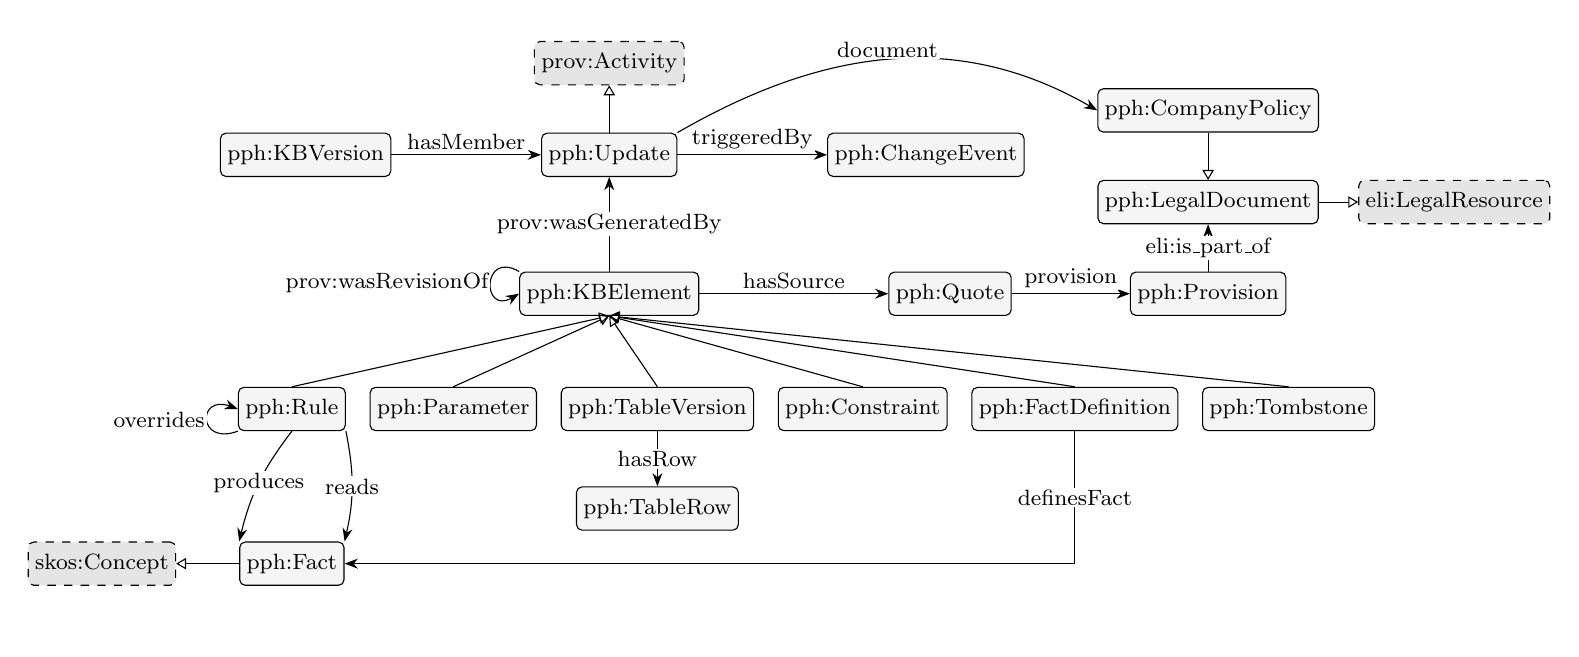
\begin{tikzpicture}[
  node distance=6mm and 7mm,
  cls/.style={draw,rounded corners=2pt,fill=gray!8,font=\footnotesize,minimum height=5.5mm,inner sep=2.5pt},
  ext/.style={cls,fill=gray!20,dashed},
  sub/.style={-{Triangle[open]},thin},
  rel/.style={-{Stealth},thin},
  lab/.style={font=\footnotesize,fill=white,inner sep=0.8pt}]

% unsur knowledge base
\node[cls] (el) {pph:KBElement};
\node[cls,below left=9mm and 22mm of el] (rule) {pph:Rule};
\node[cls,right=3mm of rule] (par) {pph:Parameter};
\node[cls,right=3mm of par] (tab) {pph:TableVersion};
\node[cls,right=3mm of tab] (con) {pph:Constraint};
\node[cls,right=3mm of con] (fd) {pph:FactDefinition};
\node[cls,right=3mm of fd] (tomb) {pph:Tombstone};
\foreach \n in {rule,par,tab,con,fd,tomb} \draw[sub] (\n.north) -- (el.south);
\node[cls,below=7mm of tab] (row) {pph:TableRow};
\draw[rel] (tab) -- node[lab]{hasRow} (row);

% fakta
\node[cls,below=14mm of rule] (fact) {pph:Fact};
\node[ext,left=8mm of fact] (concept) {skos:Concept};
\draw[sub] (fact) -- (concept);
\draw[rel] (rule.south) to[bend right=12] node[lab]{produces} (fact.north west);
\draw[rel] (rule.south east) to[bend left=12] node[lab]{reads} (fact.north east);
\draw[rel] (fd.south) |- node[lab,pos=0.25]{definesFact} (fact.east);
\draw[rel] (rule.south west) to[out=200,in=160,looseness=5] node[lab,left]{overrides} (rule.west);

% asal-usul
\node[cls,right=24mm of el] (quote) {pph:Quote};
\node[cls,right=15mm of quote] (prov) {pph:Provision};
\node[cls,above=6mm of prov] (doc) {pph:LegalDocument};
\node[ext,right=5mm of doc] (eli) {eli:LegalResource};
\node[cls,above=6mm of doc] (pol) {pph:CompanyPolicy};
\draw[rel] (el) -- node[lab,above=1pt]{hasSource} (quote);
\draw[rel] (quote) -- node[lab,above=1pt]{provision} (prov);
\draw[rel] (prov) -- node[lab]{eli:is\_part\_of} (doc);
\draw[sub] (doc) -- (eli);
\draw[sub] (pol) -- (doc);

% perubahan dan versi
\node[cls,above=12mm of el] (upd) {pph:Update};
\node[cls,left=19mm of upd] (ver) {pph:KBVersion};
\node[cls,right=19mm of upd] (ev) {pph:ChangeEvent};
\node[ext,above=6mm of upd] (act) {prov:Activity};
\draw[rel] (el) -- node[lab]{prov:wasGeneratedBy} (upd);
\draw[rel] (ver) -- node[lab,above=1pt]{hasMember} (upd);
\draw[rel] (upd) -- node[lab,above=1pt]{triggeredBy} (ev);
\draw[sub] (upd) -- (act);
\draw[rel] (upd.north east) to[out=30,in=150] node[lab,above]{document} (pol.west);
\draw[rel] (el.north west) to[out=150,in=210,looseness=5] node[lab,left]{prov:wasRevisionOf} (el.west);

\node[font=\footnotesize,align=left,anchor=north west] at ([yshift=-3mm]concept.south west)
  {\ontologicatatan};
\end{tikzpicture}

\caption{Ontology of the knowledge base. Dashed classes are reused from external vocabularies.}
\label{fig:ontology}
\end{figure*}

Calculation expressions are literal attributes of rules. The engine executes them instead of a reasoner, because tax arithmetic requires exact fractions, explicit rounding to the rupiah, and fixed-point iteration for gross-up. Listing~\ref{lst:ter} shows the stored form of the gold rule that applies TER to monthly gross income. A regulatory change therefore touches only data in the graph. The rounding rule of PER-11/PJ/2025, for example, is a new version of the parameter \texttt{pph\_round\_mode}, not a change of code.

\begin{listing}[!t]
\caption{The gold rule that applies TER to monthly gross income, as stored in the knowledge graph (prefixes shortened).}
\label{lst:ter}
\centering
\begin{minipage}{0.97\columnwidth}
\scriptsize
\begin{verbatim}
rec:229 a pph:KBElement, pph:Rule ;
  prov:wasGeneratedBy upd:GOLD-E03 ;
  pph:elementId "REG.TER.RUNNING" ;
  pph:layer pph:Regulation ;
  pph:modality pph:Mandatory ;
  pph:scope pph:Period ;
  pph:condition "not is_final_period" ;
  pph:expression
    "round(ter_rate * gross_income, 1,
           param('pph_round_mode'))" ;
  pph:produces fact:pph21_running ;
  pph:reads fact:gross_income, fact:ter_rate ;
  pph:usesParameter "pph_round_mode" ;
  pph:validFrom "2024-01-01"^^xsd:date ;
  pph:recordedOn "2023-12-27"^^xsd:date ;
  pph:hasSource rec:229/source/0, rec:229/source/1,
                rec:229/source/2 .
\end{verbatim}
\end{minipage}
\end{listing}

The validity period and the recording date make the knowledge base bitemporal, because a question asked on date $\omega$ sees only records with $t_c \leq \omega$. Fig.~\ref{fig:bitemporal} shows what this gives an employer. Employee B (status TK/0, monthly salary Rp8,000,000, employer in a labor-intensive sector eligible under PMK 10/2025) has PPh 21 of Rp125,448 in January 2025. A question asked on 31 January returns no government-borne tax, because the knowledge base does not yet contain PMK 10/2025. The same question asked on 10 February returns Rp125,448 borne by the government and paid to the employee in cash. The difference is the correction the employer owes for January.

\begin{figure}[!t]
\centering
\figBitemporal
\caption{Two time axes for Employee B. The same question about January 2025 returns the value that was correct with the knowledge of 31 January and the value that applies once PMK 10/2025 has been issued.}
\label{fig:bitemporal}
\end{figure}

\subsection{Inference Engine}
\label{sec:engine}
The engine computes one case for a full tax year (Algorithm~\ref{alg:engine}). It collects the rules that produce each fact in each period, keeps those valid in the period and recorded on or before $\omega$, and filters them by their conditions. When several rules remain, the engine applies lex superior (mandatory regulation, then company rule, then adopted optional regulation, then default), lex specialis through explicit \texttt{overrides} relations, and lex posterior. A company rule that loses to a mandatory rule with a different value is reported as a conflict. Facts are evaluated on demand with memoization, gross-up is computed as the least fixed point of the tax allowance, and the final period recomputes the year. Expressions may call only 29 registered functions, and all arithmetic is exact, so a money value that is not a whole rupiah raises an error instead of being rounded silently.

Fig.~\ref{fig:engine} follows the March 2024 withholding of Employee A through the engine. The annualized-method rule fails the validity filter, the TER rule wins, and its expression reads gross income and the TER rate. Gross income is the salary, the THR, and Rp561,000 of employer premiums; the rate is 12\% because category B and a gross of Rp30,561,000 fall in that bracket. Every value carries its rule and quotes, so the trace runs from Rp3,667,320 to the elucidation of Article 2(1) of PP 58/2023.

\begin{figure*}[!t]
\centering
\figEngine
\caption{How the inference engine computes the withholding of Employee A for March 2024: (a) rule selection, (b) on-demand evaluation of the facts the winning rule reads, and (c) the trace from the value to the provisions. All values are engine output.}
\label{fig:engine}
\end{figure*}

\begin{algorithm}[!t]
\caption{Evaluation of one case}
\label{alg:engine}
\footnotesize
\begin{algorithmic}[1]
\REQUIRE knowledge base $\K$, case $x$ (one employee, one tax year), knowledge date $\omega$
\FOR{each period $t$ of $x$ and each output fact $f$}
  \STATE $R \gets$ rules producing $f$, valid in $t$, with $t_c \leq \omega$
  \STATE $R \gets \{r \in R : \varphi_r(x, t)\}$
  \STATE $r^* \gets$ winner of $R$ by rank, then \texttt{overrides}, then recency; log a conflict if a company rule loses with a different value
  \STATE evaluate $e_{r^*}$, computing every fact it reads on demand (fixed point for gross-up)
  \STATE record value, rule, and source quotes of $f$
\ENDFOR
\STATE recompute the year in the final period of employment
\RETURN values, conflict report, trace
\end{algorithmic}
\end{algorithm}

\subsection{LLM-Assisted Knowledge Acquisition}
\label{sec:acquisition}
The acquisition pipeline turns one document into at most one update (Fig.~\ref{fig:acqflow}). The pipeline locks the document text with SHA-256, splits it by article, and trims it to a token budget. Annex tables that were extracted to files are described in the prompt, not copied. A first model call judges whether the document changes the PPh 21 computation for permanent employees and must support the judgment with verbatim quotes. A second call, repeated $m$ times independently, drafts the update as structured JSON: elements to add, change, or remove, each with a quote from its provision. The prompt carries the vocabulary of facts and functions and up to 220 related records retrieved with SPARQL, and the model never computes tax. A deterministic converter turns each draft into knowledge-base records.

\begin{figure*}[!t]
\centering
\figAcquisitionFlow
\caption{Acquisition of one document. The model drafts; deterministic gates, behavioral consensus, and a reviewer decide.}
\label{fig:acqflow}
\end{figure*}

Five gates check every draft (Table~\ref{tab:gates}). Gate G1 applies the JSON schema, strict application to the knowledge base, 14 SHACL node shapes, and 12 SHACL-SPARQL constraints. G2 requires that each quote occurs in the document and that every new number and date occurs in the quote of its element. G3 checks expressions, the dependency graph, and references. G4 is a regression test: on a set $\SG$ of generated cases, results before the effective date and results with $\omega < t_{\mathit{iss}}$ must not change. G5 requires every added or changed element to change at least one output or conflict on $\SG$; without it, an empty update passes all other gates. The set $\SG$ holds at most 300 cases, is generated from each draft without reading the gold knowledge base or the test cases, and does not overlap the test space. A draft that fails receives the gate messages and gets one repair round.

\begin{table}[!t]
\caption{Verification gates and the failures they caught among the 49 initial drafts for the 18 real documents (first failing gate; 17 drafts failed, 11 of them passed after repair).}
\label{tab:gates}
\centering\footnotesize
\setlength{\tabcolsep}{3pt}
\begin{tabularx}{\columnwidth}{@{}lLLr@{}}
\toprule
Gate & Checks & Failure observed & Drafts \\
\midrule
G1 & schema, SHACL & a validity end that is not the last day of a month (PKB Taekwang) & 2 \\
G2 & quotes, numbers, dates & a quote that is not verbatim (E03); a relief rate absent from its quote (E09) & 8 \\
G3 & expressions, references & a rule reading a table not yet valid (E10) & 1 \\
G4 & regression on $\SG$ & engine error on generated cases (E07) & 1 \\
G5 & non-vacuity & a stated effective date that changes no case (E04) & 5 \\
\bottomrule
\end{tabularx}
\end{table}

The drafts that pass are grouped by behavior. Two drafts belong to the same group when they give the same output values and the same conflict report on every case of the union of their $\SG$ sets, at both knowledge dates. The largest group wins. A tie, or no draft that passes, ends in abstention, and the document goes to the reviewer without a proposal.

\subsection{Cross-Layer Impact Analysis}
A company policy is \emph{affected} by an update when the value of a fact produced by one of its rules changes, when the winning rule of a fact it reads or produces changes, or when a new conflict appears. The detector works statically. It computes $F_\Delta$, the set of facts touched by the update and their downstream closure. It then flags each policy rule that reads a fact in $F_\Delta$ or produces a fact that a rule of the update also produces. The reviewer sees the flagged policies next to the update.

\subsection{Application and Human Review}
The application exposes both paths to payroll staff (Fig.~\ref{fig:screens}). The calculator computes one employee for a year and shows the rule and provision behind each value. A drafted update appears on the review page with its quotes, the checks on the current knowledge base, before-and-after results for a fixed set of payroll scenarios, and the affected company policies. The reviewer then approves the update, edits it, asks the model to repair it, or rejects it. A chat assistant can explain the knowledge base and prepare drafts, but only the reviewer approves.

\begin{figure*}[!t]
\centering
\begin{minipage}[b]{0.555\textwidth}\centering
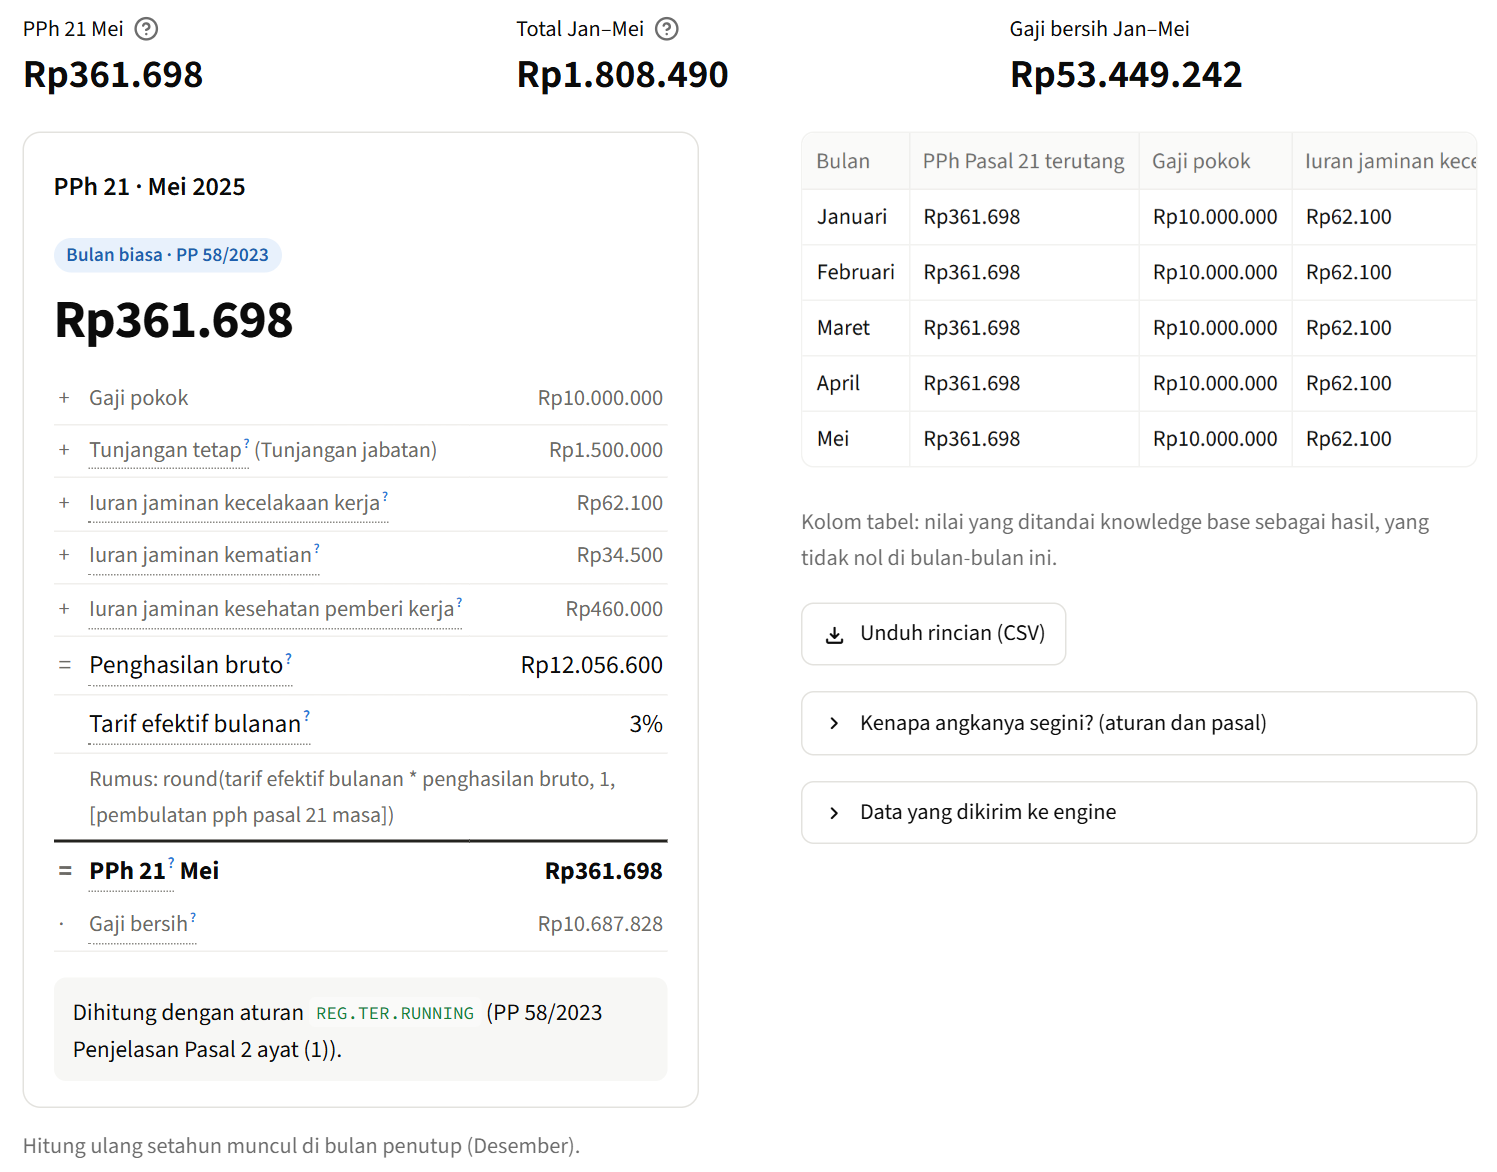
\includegraphics[width=\textwidth]{figs/screen_calculator.png}\\[1pt]{\footnotesize (a)}
\end{minipage}\hfill
\begin{minipage}[b]{0.425\textwidth}\centering
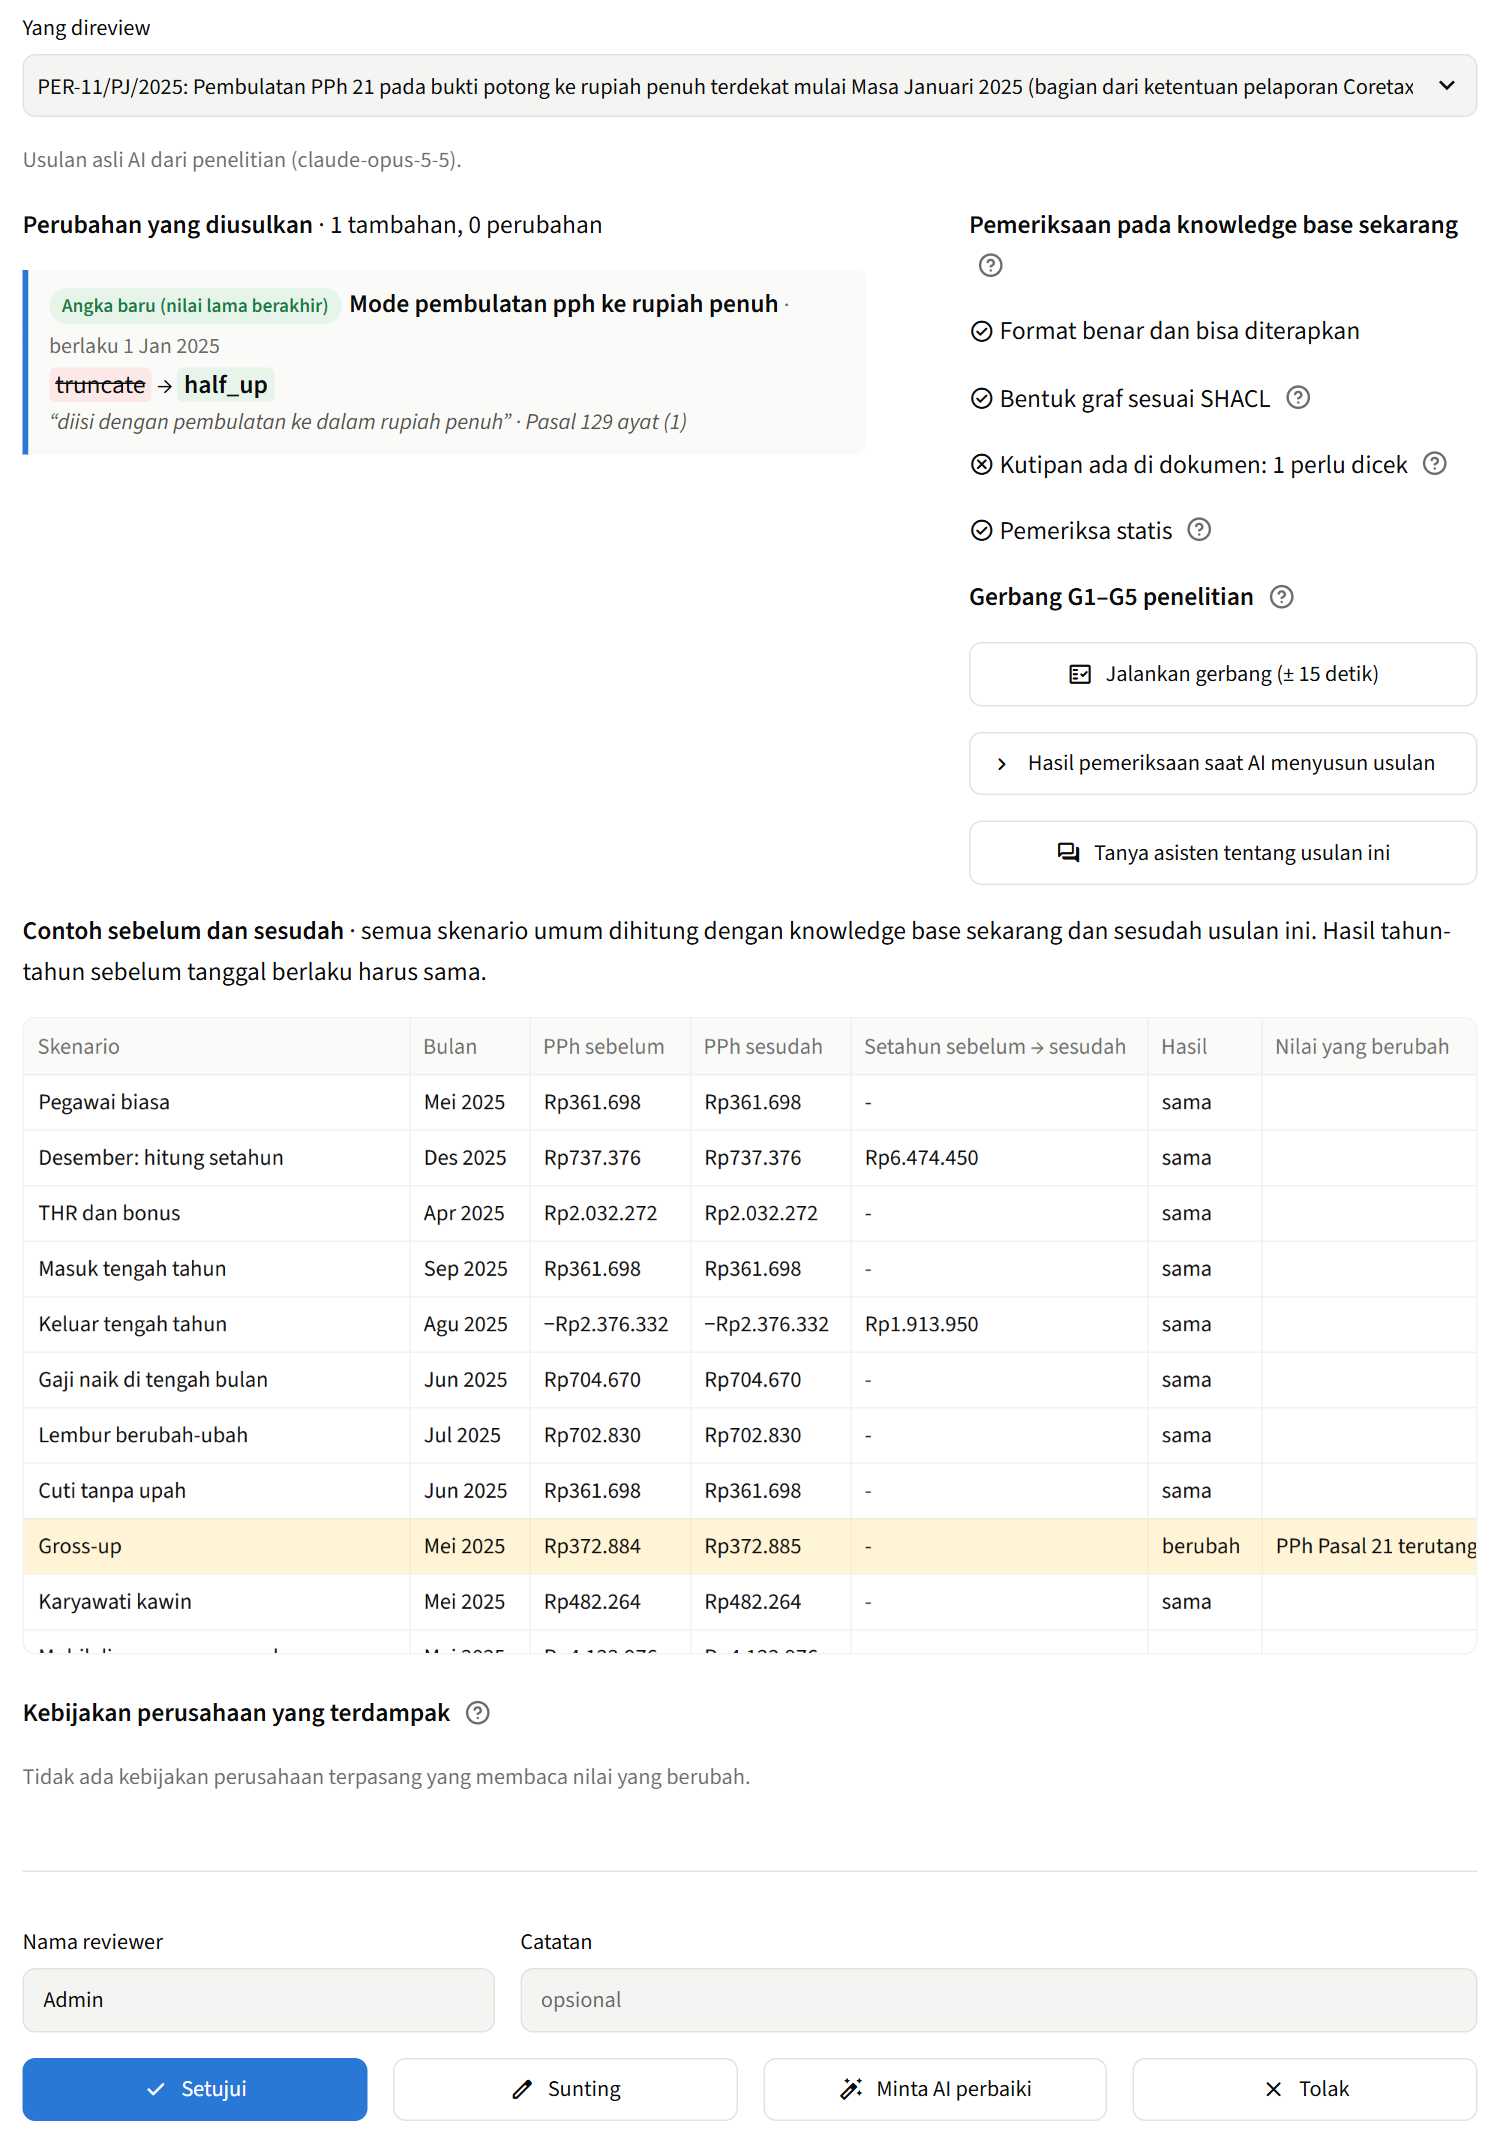
\includegraphics[width=\textwidth]{figs/screen_review.png}\\[1pt]{\footnotesize (b)}
\end{minipage}
\caption{The application, in Indonesian. (a) Calculator result for May 2025: gross income built from salary, allowance, and employer premiums, the TER rate of 3\%, PPh 21 of Rp361,698, and the rule \texttt{REG.TER.RUNNING} with its provision. (b) Review of the drafted update for PER-11/PJ/2025 (rounding mode \texttt{truncate} to \texttt{half\_up}, quoted from Article 129(1)), with the checks on the current knowledge base, before-and-after results for common scenarios (the gross-up scenario changes), affected company policies (none), and the approve, edit, repair, and reject actions.}
\label{fig:screens}
\end{figure*}

% ============================================================================
\section{Case Study: Adapting to the Effective-Rate Method}
\label{sec:casestudy}
% ============================================================================
This section follows one regulation, PP 58/2023, from its text to a traced withholding value, using the stored run of the evaluation (Fig.~\ref{fig:case}). It illustrates how the pipeline works; whether its updates are correct is assessed against the gold knowledge base in Sections~\ref{sec:design} and~\ref{sec:results}.

\begin{figure*}[!t]
\centering
\figCaseStudy
\caption{Case study of PP 58/2023 (event E03): relevance quotes, gate results of the three drafts, consensus, the selected update, and the trace of the March 2024 withholding of Employee A.}
\label{fig:case}
\end{figure*}

The relevance call quoted six provisions and judged the regulation relevant. Two of the quotes are Article 2(1), which lists the withholding rates, and Article 2(4)(a), which applies category A to monthly gross income. Three drafts followed. Draft 1 passed all five gates. Drafts 2 and 3 failed G2 because a quote attached to the TER rule did not occur verbatim in the regulation text, and both passed after one repair round. The three drafts then behaved identically on the generated cases and formed one group, so the pipeline selected draft 1. Its six model calls took 164 seconds in total and cost USD 0.60.

The selected update has three elements. A table assigns a TER category to each PTKP status, and the second element is the monthly TER table referenced from the annex of the regulation. A rule multiplies monthly gross income by the rate in every period except the final one. The gold update for the same event has seven elements, yet both give the same results on every test case, because the draft states inline what the gold update spreads over separate facts. The update sets the March 2024 withholding of Employee A to Rp3,667,320 (Table~\ref{tab:slip}) and traces it to the elucidation of Article 2(1). The annualized-method rule still exists in the knowledge base after this update, but the drafted TER rule overrides it explicitly (lex specialis) from January 2024.

The companion regulation PMK 168/2023 (event E04) ended in abstention. Its formal closing of the annualized-method rules and its new deduction for religious donations paid through the employer therefore did not enter the knowledge base. An abstention appears on the review page as a document with no proposal, which the reviewer must formalize by hand. Section~\ref{sec:res-chain} measures what happens when nobody does.

% ============================================================================
\section{Evaluation Design}
\label{sec:design}
% ============================================================================
\subsection{Properties under Test}
The evaluation tests the four properties named in Section~\ref{sec:intro}, after first validating the instruments that every later number depends on. Table~\ref{tab:evalmap} maps each property to its experiment, data, metrics, and preregistered hypothesis. Experiment E1 tests the expressiveness of the representation, E2 the safety of a single drafted update, E3 the stability of updates applied in a chain, and E4 the detection of affected company policies. E0 validates the instruments, and E5 compares the system with code maintenance and with direct calculation by an LLM.

\begin{table*}[!t]
\caption{Evaluation map: properties, experiments, data, metrics, and preregistered hypotheses. One-sided bounds are 95\% bounds.}
\label{tab:evalmap}
\centering\footnotesize
\setlength{\tabcolsep}{3pt}
\begin{tabularx}{\textwidth}{@{}P{2.7cm} P{0.6cm} P{3.4cm} L P{4.0cm}@{}}
\toprule
Property & Exp. & Data & Metrics & Hypothesis and threshold \\
\midrule
Valid instruments & E0 & four external references, mutants & agreement per observation and per case; mutation score & mutation score $\geq 0.80$ \\
Expressiveness & E1 & 16 unseen changes with 100 examples & representational adaptability (RA): share of changes expressed without engine change & H1: lower bound of RA $\geq 0.70$ \\
Safety of one update & E2 & 13 regulations and 5 labor agreements; 20 distractors & silent error rate (SER), correct application rate (CAR), abstention, selective risk & H2a: upper bound of SER $\leq 0.25$; H2b: CAR above B3 and B4, SER not worse by more than 0.10 \\
Stability of chained updates & E3 & 33 events in order, 150 cases per tax year & operational adaptability rate (OAR); triggered errors; incorrect cases at the end of the chain & H3a: lower bound of OAR $\geq 0.75$; H3b: triggered errors within the noise bound \\
Impact detection & E4 & 134 policy--event pairs & recall, precision, $F_2$ & H4a: lower bound of recall $\geq 0.70$; H4b: $F_2$ above both simple detectors \\
Comparison & E5 & two open-source calculators; 100 operational cases & days and lines of code to adopt TER; exact match of direct LLM calculation & none (descriptive) \\
\bottomrule
\end{tabularx}
\end{table*}

\subsection{Regulation Replay Protocol}
\label{sec:protocol}
The protocol replayed the 13 test events and 20 distractor documents in the order of their issue dates, 33 events in all. Isolated mode (E2) applied each draft to the gold knowledge base before its event. Chained mode (E3) applied each draft to the knowledge base that the system itself had produced. Reusing the drafts of the isolated run gives the transplanted chain, and writing the drafts again with the system's own knowledge base as context gives the regenerated chain. No reviewer intervened in either mode, so the results bound the pipeline from below, and an abstention left the knowledge base unchanged. Each chain ran once and scored 150 sampled cases per tax year, so the number of scored cases grew from 300 to 600 as tax years entered.

\subsection{Data and Temporal Split}
\label{sec:data}
The development set, used to design prompts, gates, and the selection rule, contained 13 regulatory events from 2012 to 2022, five fictional regulations, and one labor agreement. The test set contained the 13 real events of 2023--2026 (Fig.~\ref{fig:timeline}), 20 distractor documents whose correct update is empty, and five real collective labor agreements. It also contained 14 synthetic company policies, four counterfactual versions of real documents with altered values, and 16 unseen changes. Appendix~\ref{app:tables} lists the corpus with the size of each gold update. A news search found no regulation issued between the preregistration and 3 November 2026 that could be used as a prospective test.

The representation and the engine were developed after the test regulations had been published, so hindsight bias weakens the claim that those regulations need no engine change. The 16 unseen changes address this bias. A separate agent wrote them, with 5 to 7 worked examples each, and sealed them with a hash manifest before the representation was frozen. Another agent that took no part in the design then expressed them as updates.

\subsection{Ground Truth and Instrument Validation}
\label{sec:groundtruth}
Every reported number depends on the gold knowledge base $\K^\gold$ and the test cases. Four external references validated both. The first two are the official worked examples in the regulations (GT1), with a holdout opened once, and the PPh 21 calculator of the Directorate General of Taxes (GT2). The other two are 50 cases computed step by step from the regulation texts by a calculator separate from the engine (GT3) and 21 worked examples taken from clauses of the five labor agreements (GT5). Third-party implementations were collected as a fifth reference but not used for validation. Each difference was adjudicated as an error of the knowledge base, an error of the reference, or a legal ambiguity, and ambiguities were settled in 18 written interpretations. A mutation analysis measured whether the test cases detect deliberately altered rules. No human tax practitioner reviewed the gold knowledge base. Its second reader and the reviewers of the gold material were AI agents of the same model family as the model under test.

\subsection{Test Space and Coverage}
The test space holds 2,398 employee-year cases, plus 120 to 180 cases for each company policy. Each tax year has 300 operational cases sampled from provincial wage cells of Statistics Indonesia, 42 to 45 constrained combinations with full pairwise coverage, and 15 cases around the Article 17 bracket boundaries. From 2024, each year adds 321 cases around the TER boundaries. Article 17 boundaries were tested at $b-1000$, $b$, and $b+1000$ because taxable income is rounded down to thousands. Fig.~\ref{fig:coverage} shows the result. All five Article 17 brackets occur, the 35\% bracket only in six boundary cases, and 107 of the 122 TER boundaries are tested. The highest monthly gross in the test space is Rp430.3 million. The TER rates of 30\% to 34\% start at Rp454 million and therefore occur in no case.

\begin{figure}[!t]
\centering
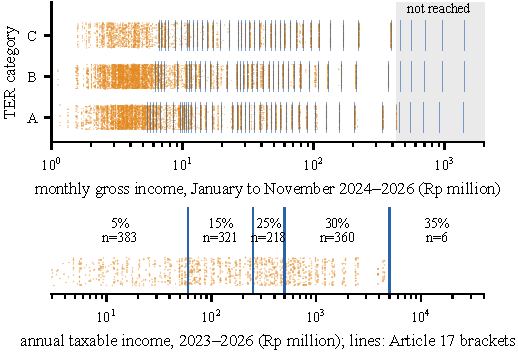
\includegraphics[width=\columnwidth]{figs/fig_coverage.pdf}
\caption{Coverage of the test space. Top: monthly gross income of every non-final TER period by category, with the TER bracket boundaries as lines; the shaded range is not reached. Bottom: annual taxable income against the Article 17 brackets, with the number of cases per bracket (1,110 cases have no taxable income).}
\label{fig:coverage}
\end{figure}

\subsection{Metrics}
\label{sec:metrics}
An update is \emph{correct} when every output value of every test case equals the value of the gold knowledge base to the rupiah at both knowledge dates and the conflict reports agree. One differing value makes it wrong. The strictness follows the use of the numbers, because withholding slips report the tax to the rupiah. Results are counted per observation (one output value of one case at one knowledge date), per tuple (one case at one knowledge date with all its observations), and per case (one employee-year).

The pipeline ends each document in one of three outcomes: a correct update, a wrong update applied without warning (a silent error), or an abstention. SER and CAR are the shares of the first two outcomes over the 18 real documents, and selective risk is SER/(SER + CAR)~\cite{xin2021abstention}. Pass@1, pass@$m$, and 1@$m$ describe the drafts before selection~\cite{chen2021evaluating,li2022alphacode}. RA is the share of unseen changes for which an update reproduces all examples without engine change. OAR is the share of chained events that add no new incorrect case, and the triggered errors of Section~\ref{sec:errortypes} are counted against a noise bound estimated from two independent isolated runs. Impact detection uses recall, precision, and $F_2$ over policy--event pairs, weighting recall because a missed affected policy costs more than a false alarm.

Four exploratory measures were added after the main results. Two describe a wrong update, namely the materiality of each wrong value (exact, within Rp1, within Rp1,000, or larger) and the number of employees it affects. The other two are the element-level precision and recall of a selected update against the gold update and the summed duration of the model calls that drafted an update.

\subsection{Baselines and Ablations}
Two baselines bracket the selection rule. B3 applies the first draft that passes G1 and G2, the pattern of one model call with validation used by single-state formalization~\cite{veeramani2026neurosymbolic,yadamsuren2026formalization}. B4 takes the majority vote of all drafts without gates, the behavioral selection of Gogani-Khiabani et al.~\cite{goganikhiabani2025maintaining}. Two simpler detectors are the baselines for impact detection: B5(i) flags every policy that touches the facts in $F_\Delta$, and B5(ii) scans the text of the policy expressions without the graph. E5 adds two external comparisons, the commit histories of open-source PPh 21 calculators (B1) and an LLM that computes the tax directly from the case data (B2). The ablations remove the knowledge-base context from the prompt, remove each gate in turn or keep only G1, and remove the repair round. Further ablations replace consensus with the first passing draft or with perfect selection, formalize a whole legal state from scratch, and remove SHACL from G1.

\subsection{Statistical Analysis and Preregistration}
Proportions are reported with exact Clopper--Pearson confidence intervals (CIs) and one-sided 95\% bounds. Paired comparisons of CAR use the exact McNemar test with Holm correction, and noninferiority of SER uses the Newcombe CI of the paired risk difference with a margin of 0.10. Each threshold was set at or above the best bound the planned sample can reach; with 18 documents and no error, the exact upper bound of SER is 0.153. McNemar reaches 80\% power with $N = 18$ only for a CAR difference near 0.45, so a failure to reject is not evidence of equivalence. Impact detection uses a bootstrap clustered by event.

The hypotheses, thresholds, data split, main test cases, analysis plan, pipeline, and engine were committed to the public repository (commit \texttt{c5983ff}) before the first test event ran. A git commit is weaker evidence than registration with a third party. The 17 targeted cases of the mutation analysis entered after the first E2 call but before any E2 result was scored. An amendment written after early results (commit \texttt{2df0727}) added the remaining nine distractors, a second isolated run, the regenerated chain, the counterfactuals, the synthetic policies, the ablation without knowledge-base context, a second model, and a sensitivity run with $m = 5$. Apart from the distractors, the second run, and the regenerated chain, the results that rest on the amendment are marked exploratory.

\subsection{Implementation and Cost}
The engine, gates, and pipeline are written in Python, the knowledge graph runs in GraphDB 11.5 with SHACL validation, and the application uses Streamlit. The main model was Claude Opus 5.5, with medium reasoning effort for relevance and high effort for drafting. Its calls used structured JSON output, prompt caching, a limit of 32,000 output tokens, and the provider's default sampling settings. The second model was \texttt{gpt-6.1-sol}. Drafting used $m = 3$ for regulations and $m = 2$ for labor agreements. The experiment calls ran on 28 and 29 October 2026 and were logged in full, so every analysis can be repeated without calling a model. The experiments cost about USD 81.6 for Claude and USD 8.1 for the second model.

% ============================================================================
\section{Results}
\label{sec:results}
% ============================================================================
Table~\ref{tab:verdicts} gives the verdict on every preregistered hypothesis; the subsections that follow report the evidence in the order of the four properties.

\begin{table*}[!t]
\caption{Hypotheses and verdicts. $^{\mathrm{a}}$Rests on the amendment written after early results.}
\label{tab:verdicts}
\centering\footnotesize
\setlength{\tabcolsep}{4pt}
\begin{tabularx}{\textwidth}{@{}P{5.2cm} L P{3.9cm}@{}}
\toprule
Hypothesis & Result & Verdict \\
\midrule
Invariants A1 and A3$_\omega$ & no violation & met \\
H1: lower bound of RA $\geq 0.70$ & 16/16 (lower bound 0.829); 15/16 (0.736) counting only the first attempt; 8/16 (0.279) without aligning the rounding convention of the examples & accepted, conditional on the rounding convention \\
H2a: upper bound of SER $\leq 0.25$ & SER 3/18, upper bound 0.377 & not accepted \\
H2b: CAR of the pipeline above B3 and B4 & 8/18 against 8/18 and 9/18; McNemar $p = 0.75$ and $p = 1.0$; Holm-adjusted $p = 1$ & not accepted \\
H2b: SER not worse by more than 0.10 & against B3, difference $-0.222$ with upper bound 0.004; against B4, difference 0 with upper bound 0.153 & met against B3, not against B4 \\
H3a: lower bound of OAR $\geq 0.75$ & transplanted chain 31/33 (0.821), mostly through masking; regenerated chain$^{\mathrm{a}}$ 23/33 (0.540) & accepted in the registered analysis, not robust \\
H3b: triggered errors within the noise bound & 29 cases on the regenerated chain$^{\mathrm{a}}$ against a noise bound of 0 & not supported \\
H4a: lower bound of recall $\geq 0.70$ & recall 0.91, cluster CI 0.75--1.00 & accepted \\
H4b: $F_2$ of the detector above B5(i) and B5(ii) & $+0.193$ (CI 0.062--0.400) against B5(ii); $-0.006$ (CI $-0.110$ to 0.058) against B5(i) & not accepted \\
\bottomrule
\end{tabularx}
\end{table*}

\subsection{Instrument Validity}
\label{sec:res-instruments}
The gold knowledge base agreed with the independent calculation on all 50 GT3 cases and all 2,107 of their observations. Its remaining differences from the other references are one-rupiah rounding and errors in the official examples. The others come from a labor-agreement clause that the knowledge base does not formalize and from examples dated before an agreement took effect (Table~\ref{tab:refs} in Appendix~\ref{app:tables}). The DJP calculator matched 15 of 20 monthly cases and all 90 final-period rows; on the other five monthly cases it differed by Rp1, because it truncates fractions where the knowledge base rounds. The development examples of GT1 matched on 22 of 26 cases, and the 13 material differences are errors in the official examples.

One of the official examples shows why adjudication is needed. The example in PMK 10/2025 caps the occupational expense of an employee who works part of the year month by month, at Rp4,550,000. The examples in PMK 168/2023 and PMK 105/2025 apply an annual cap of Rp4,750,000 to the same situation, and the knowledge base follows them. The GT1 holdout first matched 6 of 10 cases and 221 of 235 observations and exposed two errors in the gold knowledge base. It matched 8 of 10 cases and 232 of 235 observations after the correction, and its two remaining material differences concern how pension contributions were mapped. Adding 17 targeted cases raised the mutation score over nonequivalent mutants from 0.90 to 1.00. The second reader agreed on the values of 90\% of the gold units, with a Krippendorff's $\alpha$ of 0.79 for the start dates of added elements and 0.61 over all units.

\subsection{Expressiveness of the Representation}
\label{sec:res-expressiveness}
All 16 unseen changes were expressed as updates without changing the engine, and their 100 examples with 2,609 values were reproduced exactly (RA 16/16, CI 0.794--1.000, one-sided lower bound 0.829). Fifteen changes succeeded at the first attempt. The result depends on one convention update, because the examples round withholding down, like the DJP calculator, whereas the knowledge base rounds to the nearest rupiah under PER-11/PJ/2025. Eight of the 16 changes pass without that update. The other 8 differ by at most Rp11, and part of the failure of U14 comes from an update that did not state its own rounding. The changes also exposed limits that need engine functions (Table~\ref{tab:unseen} in Appendix~\ref{app:tables}). The expression language has no date arithmetic and no string construction, a company rule cannot replace a mandatory fact, and a condition cannot test a case attribute that the case data do not contain.

\subsection{Single-Document Acquisition}
\label{sec:res-single}
The pipeline applied a correct update to 8 of the 18 real documents, a wrong update to 3, and abstained on 7 (Fig.~\ref{fig:acq}(a)). SER is 0.167 (CI 0.036--0.414; upper bound 0.377) and CAR is 0.444 (CI 0.215--0.692). The first draft that passed G1 and G2 (B3) was silently wrong on 7 documents and correct on 8. Consensus therefore lowered the silent errors as a point estimate (one-sided McNemar $p = 0.0625$) without adding a correct update. The majority vote without gates (B4) was wrong on 3 and correct on 9. The pipeline was correct on 8 of the 13 regulations, wrong on 3 (E02, E07, E11), and abstained on 2 (E04, E06). It abstained on all five labor agreements, and no labor agreement was correct under any condition. A second isolated run on the 13 regulations gave 8 correct updates, 2 wrong ones, and 3 abstentions, with E07 and E11 wrong again. The second model showed the same pattern, with SER 3/18 against 7/18 for its own B3.

\begin{figure*}[!t]
\centering
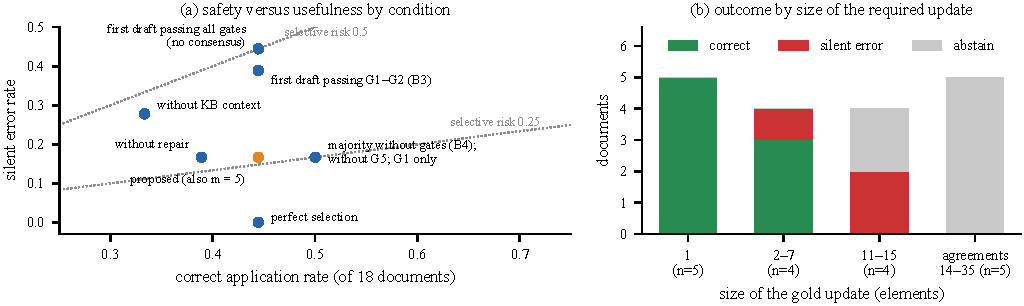
\includegraphics[width=\textwidth]{figs/fig_acquisition.pdf}
\caption{Single-document acquisition on the 18 real documents (13 regulations and 5 collective labor agreements). (a) Silent error rate against correct application rate for each condition; dotted lines mark equal selective risk. (b) Outcome of the pipeline by the number of elements in the gold update.}
\label{fig:acq}
\end{figure*}

Success depended on how much an update had to change (Fig.~\ref{fig:acq}(b)). All five documents whose gold update has one element were applied correctly, and three of the four with 2 to 7 elements. None of the four regulations with 11 to 15 elements was, and neither was any of the five labor agreements with 14 to 35 elements. By change type, 4 of the 5 parameter changes (T1) and 4 of the 8 structural regulations were correct.

The three silent errors are material. Every wrong withholding value differs from the gold value by more than Rp1, and most by more than Rp1,000. The update for E02 (benefits in kind) affected 52 employee-year cases, with a largest withholding difference of Rp61,573,500 and a median relative difference of 19.7\%. The update for E07 (premium relief) affected 42 cases, with a largest difference of Rp279,300, and the update for E11 (government-borne tax for 2026) affected 2 cases, with a largest difference of Rp39,650. Element-level similarity to the gold update did not predict correctness. Five correct updates match their gold update element for element, while the correct update for E03 recovers 3 of 7 gold elements and the correct update for E10 matches none. The wrong updates recover between 13\% and 50\% of the gold elements. Several equivalent updates can state the same regulation, which is why correctness is judged on computed results.

The drafts themselves were often right. The drafts before selection reached pass@1 of 0.667, pass@$m$ of 0.692, and 1@$m$ of 0.615 on the regulations, so consensus did not beat a randomly chosen draft. Of the 49 initial drafts, 17 failed a gate (Table~\ref{tab:gates}) and 11 of those passed after repair. All 18 real documents were judged relevant. Of the 20 distractors, 7 were judged relevant (0.35, CI 0.15--0.59), but only P01 led to a wrong update. Exploratory results complete the picture. The four counterfactual documents gave 1 correct update, 1 wrong update, and 2 abstentions, and no draft reproduced the original value of a counterfactual parameter (0 of 6). The pipeline was correct on 5 of the 14 synthetic policies, wrong on 6, and abstained on 3. Of 28 quotes checked by hand, 23 supported their element and 5 supported it partly.

\subsection{Component Ablation}
\label{sec:res-ablation}
Table~\ref{tab:ablation} isolates the components. Removing the knowledge-base context from the prompt raised the silent errors from 3 to 5 and lowered the correct updates from 8 to 6. Removing G2, G3, or G4 changed no outcome, and keeping only G1 or removing G5 turned one abstention, E04, into a correct update. G5 rejected all three drafts for E04 because their stated effective date, 1 January 2024, changed no generated case in that month. Two of them also carried an element without effect, such as a rule that restated an existing one. Without G5, the consensus of these drafts was correct on the test cases. The three silent errors passed every gate configuration. The reduction of silent errors from 8 for the first passing draft to 3 for the pipeline therefore comes from drawing several drafts and requiring their agreement. The gates did not lower it further on these 18 documents. Perfect selection among the drafts that passed the gates would have removed the three silent errors but added no correct update, so every correct draft that survived the gates was already chosen.

\begin{table}[!t]
\caption{Ablation on the 18 real documents (correct, silent error, abstain). $^{\mathrm{a}}$Amendment. $^{\mathrm{b}}$Recomputed after the main results from the stored drafts, without new model calls.}
\label{tab:ablation}
\centering\footnotesize
\setlength{\tabcolsep}{3pt}
\begin{tabularx}{\columnwidth}{@{}Lccc@{}}
\toprule
Condition & Correct & Silent & Abstain \\
\midrule
Full pipeline & 8 & 3 & 7 \\
Without knowledge-base context$^{\mathrm{a}}$ & 6 & 5 & 7 \\
Without G2$^{\mathrm{b}}$ & 8 & 3 & 7 \\
Without G3$^{\mathrm{b}}$ & 8 & 3 & 7 \\
Without G4 & 8 & 3 & 7 \\
Without G5 & 9 & 3 & 6 \\
G1 only$^{\mathrm{b}}$ & 9 & 3 & 6 \\
Without the repair round & 7 & 3 & 8 \\
Majority vote without gates (B4) & 9 & 3 & 6 \\
First draft passing G1--G2 (B3) & 8 & 7 & 3 \\
First draft passing all gates & 8 & 8 & 2 \\
Perfect selection & 8 & 0 & 10 \\
\bottomrule
\end{tabularx}
\begin{minipage}{\columnwidth}\vspace{2pt}\scriptsize
SHACL in G1 rejected 7 of 319 drafts that had passed the JSON schema. Formalizing a whole legal state from scratch produced no draft that passed the gates, from six drafts on two legal states.
\end{minipage}
\end{table}

\subsection{Chained Replay, 2023--2026}
\label{sec:res-chain}
On the transplanted chain, 31 of 33 events added no new incorrect case (OAR CI 0.798--0.993), which meets H3a (Fig.~\ref{fig:replaychain}). It meets H3a only because new errors appeared at two events, E02 with 15 cases and the distractor P01 with 264 cases. Already 279 of 300 scored cases were wrong after P01, and the count rose to 579 of 600 only because cases of later tax years were added. The high OAR therefore reflects masking, since later events could not add errors to cases that were already wrong.

\begin{figure*}[!t]
\centering
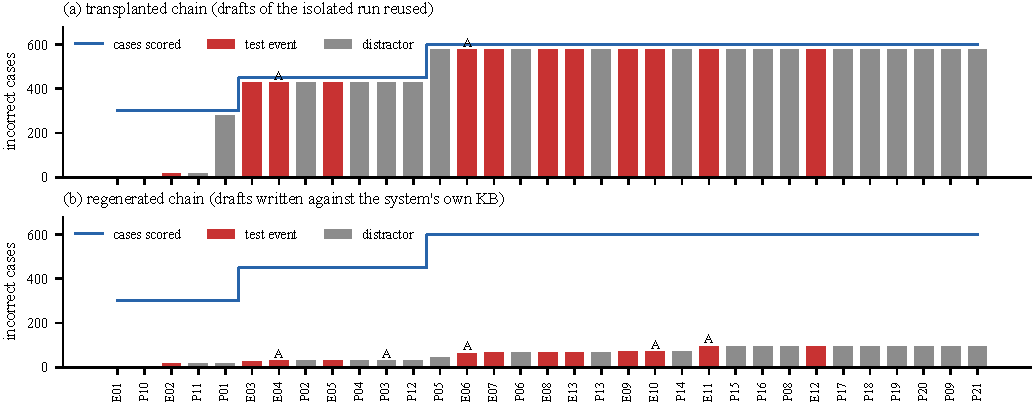
\includegraphics[width=\textwidth]{figs/fig_replay.pdf}
\caption{Regulation replay in chronological order. Bars give the incorrect employee-year cases after each event (red: test event, grey: distractor); the line gives the number of cases scored, which grows as tax years enter; A marks an abstention. Each chain was run once.}
\label{fig:replaychain}
\end{figure*}

The regenerated chain follows Definition~\ref{def:adapt} fully and gives a different picture. Its OAR is 23/33 (CI 0.513--0.844), only 5 of the 13 regulatory events added no new error, and 93 of 600 cases were wrong at the end. Of the 103 new errors, 53 appeared at events where the chain abstained; the abstention on E04 alone added 8. Triggered errors totalled 29 cases on the 13 regulatory events (57 with the distractors), and 26 of them occurred at E10 and E11, where the chain had abstained. Most errors in the chain therefore came from a knowledge base that stayed out of date, not from a wrong update that spread.

\subsection{Cross-Layer Impact Detection}
Of the 134 policy--event pairs, 33 were affected (prevalence 0.25), and 27 of these involved synthetic policies. The frozen detector reached a recall of 0.91 (cluster CI 0.75--1.00), a precision of 0.71, and an $F_2$ of 0.862. Its $F_2$ exceeded that of scanning the policy text without the graph, B5(ii), at 0.669, but not that of flagging every policy that touches $F_\Delta$, B5(i), at 0.868. The three missed pairs involve a policy that produces a fact which changes through an upstream parameter. A second version of the detector, written after these results, closes that gap and becomes identical to B5(i). The execution-based labels and a manual labeling of conflicts agreed poorly (Cohen's $\kappa = -0.018$) because one records a change of value and the other a breach of a rule.

\subsection{Comparison with Code Maintenance and Direct LLM Calculation}
\label{sec:res-compare}
The TER regime consists of 8 new and 13 changed elements of the knowledge base across E03 and E04, with no engine change. Two open-source PPh 21 calculators added TER 26 and 915 days after PP 58/2023 was issued, changing 163 and 504 lines of code (Fig.~\ref{fig:adapt}). The model calls that drafted the two updates took about 12.5 minutes in total, 164 seconds for E03 and 586 seconds for E04. The median over the 18 real documents was about two minutes. Review time was not measured, and the delays of the calculators include development and release practices that this comparison does not control, so the comparison is descriptive. An LLM that computed PPh 21 directly from the case data (B2, exploratory) was exact on 76 of 100 operational cases (CI 0.66--0.84) and within Rp1 on 97. It gave no trace and cost USD 0.068 per case for every computation, whereas the pipeline pays once per document.

\begin{figure}[!t]
\centering
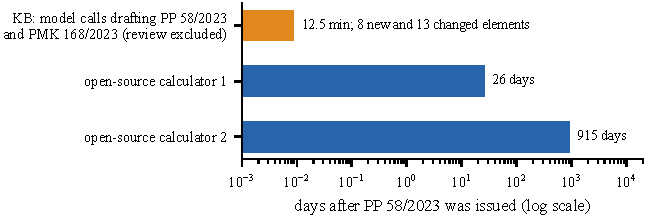
\includegraphics[width=\columnwidth]{figs/fig_adapt.pdf}
\caption{Time to adapt to the TER method after PP 58/2023 was issued: summed duration of the model calls that drafted the knowledge updates (review time not measured) against the commits of two open-source calculators, with the size of each change.}
\label{fig:adapt}
\end{figure}

% ============================================================================
\section{Discussion}
\label{sec:discussion}
% ============================================================================
\subsection{When Can an LLM-Drafted Update Be Trusted?}
The representation held: every unseen change and every real event could be expressed as data, and a structural change such as TER became 21 records instead of new code. The acquisition pipeline held only for small updates. Single-element parameter changes, such as the yearly pension wage cap, were drafted correctly every time, while no document that needed 11 or more elements was, and the five labor agreements ended in abstention. With an upper bound of 0.377 on the silent error rate and silent errors that moved withholding by up to Rp61.6 million, the pipeline cannot run without a reviewer. Drawing several drafts and requiring their agreement cut the silent errors from 7 or 8 to 3. The reduction came from more abstentions, not from more correct updates, and the agreement could not catch errors on which all drafts agreed.

These figures are stricter than those of related systems because the unit differs. Veeramani et al.\ report 80\% accuracy over 20 scenarios~\cite{veeramani2026neurosymbolic} and Jurayj et al.\ 75 correct answers of 100 cases~\cite{jurayj2026tax}, both per computed case. Here an update counts as correct only when all test cases at both knowledge dates match the gold knowledge base, which is the standard a payroll department needs before it accepts a rule change.

\subsection{Why LLM Updates Fail}
Table~\ref{tab:taxonomy} counts the failures by kind. The gates caught failures of form: quotes that were not verbatim, numbers absent from their quotes, schema violations, dangling references, and an engine error. The silent errors were failures of content that no gate inspects. The update for E02 had three elements, and only two of them match elements of the 15-element gold update. It left out the exemption ceilings for housing, gifts, sports facilities, and vehicles, as well as the gross-up of tax borne by the employer. The update for E11 tested the Rp10 million eligibility ceiling against taxable benefits after exemptions instead of the value of housing and vehicle benefits. The update for E07 read the regulation correctly but conditioned the relief on a case attribute that the case data do not contain; with the attribute renamed, the same update is correct on every tuple. That error is an interface problem. The prompt lists the facts and functions of the knowledge base but not the attributes of the case data, so the model had to invent a name. E07 and E11 were wrong again in the second run, with drafts that agreed, which explains why consensus did not catch them. No fabricated quote and no memorized value of a counterfactual parameter was observed.

\begin{table}[!t]
\caption{Failures of the drafted updates on the 18 real documents and 20 distractors, by kind, and the component that caught them.}
\label{tab:taxonomy}
\centering\footnotesize
\setlength{\tabcolsep}{3pt}
\begin{tabularx}{\columnwidth}{@{}LlL@{}}
\toprule
Kind of failure & Count & Caught by \\
\midrule
Incomplete update (missing exemptions) & 1 document (E02) & none (silent) \\
Wrong scope of an income base & 1 document (E11) & none (silent) \\
Case attribute absent from the data & 1 document (E07) & none (silent) \\
Distractor applied as a change & 1 of 20 (P01) & none (silent) \\
Quote or number not grounded in the text & 8 drafts & G2 \\
Element or effective date without effect & 5 drafts & G5 \\
Schema or SHACL violation & 2 drafts & G1 \\
Reference to a table not yet valid & 1 draft & G3 \\
Engine error on generated cases & 1 draft & G4 \\
\bottomrule
\end{tabularx}
\begin{minipage}{\columnwidth}\vspace{2pt}\scriptsize
Draft counts refer to the first failing gate of the 49 initial drafts. The five G5 failures include all three drafts of E04; without G5, their consensus was correct on the test cases.
\end{minipage}
\end{table}

\subsection{Implications for Payroll Practice}
Three practices follow from the results. Every abstention must enter a review queue, because the chain showed that an unprocessed document becomes errors in later periods: 53 of the 103 new errors on the regenerated chain arose at abstentions. A reviewer of a drafted update needs to see who is affected, not only that the gates passed, since the three silent errors passed every gate. The before-and-after scenarios and the impact report of Fig.~\ref{fig:screens} show this. Retroactive regulations call for both time axes, so that the system can list the corrections owed for periods that were correct when they were paid, as Fig.~\ref{fig:bitemporal} does for January 2025. Structural regulations, updates with more than a few elements, labor agreements, and documents that resemble distractors should not be applied without a full review. The system supports the reviewer and does not give tax advice; the employer remains responsible for every withholding.

\subsection{Implications for Knowledge-Based Systems and Legal AI}
Splitting the knowledge into a graph for structure and provenance and expressions for arithmetic let a change of method, a change of rounding, and a retroactive facility all enter as data. The engine meanwhile kept exact arithmetic and a trace to the provisions. The replay protocol does not depend on PPh 21. Any executable legal rule base with dated documents and a gold history can be replayed in isolation and in a chain. The split into inherited, new, and triggered errors then separates a stale knowledge base from a wrong update. Applying the protocol to another tax or jurisdiction requires a new gold history and test space, which carried most of the cost of this study. The results suggest seven design rules for LLM-assisted maintenance of such a rule base:
\begin{enumerate}
\item require a verbatim quote for every number and date in a drafted element;
\item draw several independent drafts and allow abstention;
\item route every abstention to a reviewer queue;
\item check the scope and completeness of an update against the provisions it cites, which no gate in this study did;
\item give the model the attributes of the case data and warn when a draft introduces a new one, the lesson of E07;
\item report an element or effective date without effect to the reviewer instead of rejecting the whole draft, the lesson of E04;
\item evaluate updates by chronological replay rather than on a single legal state.
\end{enumerate}

\subsection{Threats to Validity}
Internal validity is limited because the same party wrote the gold knowledge base, the engine, and the interpretations. It is also limited because AI agents of the same model family as the tested model drafted and reviewed the gold material and the unseen changes, and no human tax practitioner validated them. The official examples, the DJP calculator, the holdout, and separate engine tests mitigate this risk without removing it.

The analysis is not fully blind. The amendment was written after early results, and the gates were adjusted during development until the gold updates of the test events passed them. The gold synthetic policies were corrected after the model output was visible, which raised the result of the pipeline on those policies from 3 correct and 8 wrong to 5 correct and 6 wrong. Agreement with a reference is not the same as conformity with the law, which limits construct validity~\cite{witt2024encoding}. External validity is limited to one jurisdiction, one tax, five labor agreements, and two model families. Eighteen documents, one run per chain, and $m$ of 3 and 2 limit conclusion validity. Contamination cannot be tested with a cutoff split, because every test event was issued before the training cutoff of both models; the evidence against memorization comes only from the counterfactuals and the fictional development regulations. The headline result for expressiveness depends on aligning the rounding convention of the examples.

\subsection{Limitations}
Fifteen TER boundaries and the TER rates of 30\% to 34\% are untested, so the results do not cover monthly gross income above about Rp450 million. The 35\% Article 17 bracket occurs only in six boundary cases. Repeal without replacement (T8) has no real example. The impact detector was evaluated with the gold updates as input, so it measures the detector rather than the full pipeline. The review step itself was not studied: review time, the errors a reviewer catches, and the burden of the review queue are unmeasured, and a user study with payroll staff remains to be done. The system computes one employee at a time and does not produce withholding slips.

% ============================================================================
\section{Conclusion}
\label{sec:conclusion}
% ============================================================================
This paper built an adaptive knowledge-based system for PPh 21. Regulations and company policies form a bitemporal two-layer knowledge graph, and a deterministic engine computes the tax with a trace to the provisions. Gates, consensus, and a reviewer filter the knowledge updates that a language model drafts. Replaying the regulatory changes of 2023--2026 showed that the representation can express every change examined without modifying the engine, including 16 changes unseen by its designers once their rounding convention was aligned. The language model drafted correct updates for 8 of 18 real documents and silently wrong ones for 3. It succeeded on every single-element parameter change and failed or abstained on every document that needed 11 or more elements, including all five collective labor agreements. Most errors in a chain without review came from documents on which the system abstained, so an abstention is safe only if a person acts on it. The impact detector reached a recall of 0.91 but did no better than simple flagging.

The next step is validation of the gold knowledge base by human tax practitioners. Further work concerns a gate that checks the scope and completeness of an update, case attributes in the model's context, and a measured review workflow with payroll staff. The untested TER brackets and repeated chains with gates calibrated without the test gold data also remain.


\section*{Data and Code Availability}
The code, gold knowledge base, corpus, test space, experiment logs including every model call, analysis scripts, and the scripts that generate the figures are available at \url{https://github.com/obikastanya/pph_payroll_with_knowledge_base}. The texts of the collective labor agreements and the prompts that contain them are excluded because the agreements belong to third parties, so the company-policy runs cannot be repeated from the archive alone. Indonesian regulations are not protected by copyright (Law 28/2014, Article 42). The study involved no human subjects and no personal data; test employees are synthetic and were generated from published wage cells of Statistics Indonesia.

\appendices
% ============================================================================
% Appendices (in-paper). Supplementary material outside the article: full prompts and the values of every
% acquisition condition; per-event results; the preregistration and its amendment; statistical details and power.
% ============================================================================
\section{Notation and Glossary}
\label{app:glossary}
\begin{table}[!h]
\caption{Notation and Indonesian terms used in the article.}
\label{tab:glossary}
\centering\footnotesize
\setlength{\tabcolsep}{3pt}
\begin{tabularx}{\columnwidth}{@{}lL@{}}
\toprule
Term & Meaning \\
\midrule
$\K$, $\K^\gold$, $\K^{\mathrm{sys}}$ & knowledge base; gold knowledge base; knowledge base produced by the system \\
$\Delta$, $\hat{\Delta}$, $\Delta^\gold$ & update; update selected by the pipeline; gold update \\
$x$, $t$, $\omega$ & case (one employee-year); tax period; knowledge date \\
$\SE$, $\SG$ & test space; cases generated for the gates of one draft \\
PPh 21 & Income Tax Article 21, withheld monthly by the employer \\
PTKP & nontaxable income amount by family status (e.g., K/1: married, one dependent) \\
PKP & annual taxable income, rounded down to thousands \\
TER & average effective rate applied to monthly gross income from 2024 \\
DTP & income tax borne by the government \\
THR & religious holiday allowance \\
PKB & collective labor agreement \\
PP, PMK, PER & Government Regulation; Minister of Finance Regulation; Director General Regulation \\
DJP & Directorate General of Taxes \\
\bottomrule
\end{tabularx}
\end{table}

\section{Conflict Taxonomy}
\label{app:taxonomies}
A company rule conflicts with the regulation layer when it loses to a mandatory rule with a different value or violates a mandatory constraint. Table~\ref{tab:conflicts} lists the ten conflict types; only C4 has a real instance in the corpus, the latent conflict of Section~\ref{sec:policies}, and the synthetic policies instantiate the others.

\begin{table}[!h]
\caption{Conflict types between company policies and mandatory provisions.}
\label{tab:conflicts}
\centering\footnotesize
\setlength{\tabcolsep}{3pt}
\begin{tabularx}{\columnwidth}{@{}lL@{}}
\toprule
Code & Conflict \\
\midrule
C1 & income classified differently (regular or irregular, taxable or not) \\
C2 & a component of gross income omitted, such as employer premiums \\
C3 & a deduction that is not allowed or exceeds its ceiling \\
C4 & a government facility not passed on to employees \\
C5 & a rate or method that is no longer valid \\
C6 & an outdated parameter \\
C7 & social-security contributions split differently \\
C8 & a contribution wage cap or ceiling ignored \\
C9 & rounding that deviates from the regulation \\
C10 & a minimum entitlement breached \\
\bottomrule
\end{tabularx}
\end{table}

\section{Gate Specification}
\label{app:gates}
G1 parses a draft against the JSON schema of updates, applies it strictly to a copy of the knowledge base, and validates the result against 14 SHACL node shapes and 12 SHACL-SPARQL constraints. G2 locates each quote in the locked document text after normalizing whitespace and recognized OCR errors in digits. It requires every new number of 100 or more, every new rate, and every date of an element to occur in a quote of that element. The recording date must equal the issue date of the document. G3 parses every expression, checks that every fact, parameter, and table it reads has a valid producer in the periods concerned, and rejects cycles. G4 generates up to 300 cases from the draft itself by varying the attributes, thresholds, and periods that the draft mentions. Results before the effective date and for knowledge dates before the issue date must not change. G5 removes each added or changed element in turn and requires at least one output value or conflict on the generated cases to change. The stated effective date must also change at least one case in that month.

\section{Test Corpus and Additional Results}
\label{app:tables}
Table~\ref{tab:corpus} lists the test events, Table~\ref{tab:refs} the agreement of the gold knowledge base with the external references, and Table~\ref{tab:unseen} the unseen changes.

\begin{table}[!h]
\caption{Test corpus. $|\Delta^\gold|$ counts the added, changed, and removed elements of the gold update.}
\label{tab:corpus}
\centering\footnotesize
\setlength{\tabcolsep}{3pt}
\begin{tabularx}{\columnwidth}{@{}lLlr@{}}
\toprule
ID & Document & Type & $|\Delta^\gold|$ \\
\midrule
E01 & pension wage-cap letter 2023 & T1 & 1 \\
E02 & PMK 66/2023 (benefits in kind) & T3 & 15 \\
E03 & PP 58/2023 (TER) & T2, T7 & 7 \\
E04 & PMK 168/2023 (TER guidance) & T7, T3 & 14 \\
E05 & pension wage-cap letter 2024 & T1 & 1 \\
E06 & PMK 10/2025 (DTP, labor-intensive industry) & T4 & 15 \\
E07 & PP 7/2025 (work-accident premium relief) & T1 & 2 \\
E08 & pension wage-cap letter 2025 & T1 & 1 \\
E09 & PP 36/2025 (extension of the relief) & T6 & 2 \\
E10 & PMK 72/2025 (DTP, tourism)~\cite{pmk72_2025} & T5 & 5 \\
E11 & PMK 105/2025 (DTP 2026)~\cite{pmk105_2025} & T4 & 11 \\
E12 & pension wage-cap letter 2026 & T1 & 1 \\
E13 & PER-11/PJ/2025 (rounding) & T9 & 1 \\
\midrule
P01--P21 & 20 distractors (numbering skips P07) & -- & 0 \\
-- & 5 collective labor agreements & T10 & 14--35 \\
-- & 14 synthetic company policies & T10 & 1--7 \\
-- & 4 counterfactual documents & T1, T3, T4 & -- \\
U01--U16 & 16 unseen changes & T1--T10 & 1--21 \\
\bottomrule
\end{tabularx}
\end{table}

\begin{table}[!h]
\caption{Agreement of the gold knowledge base with external references, per observation, with the materiality of the differences.}
\label{tab:refs}
\centering\footnotesize
\setlength{\tabcolsep}{2.5pt}
\begin{tabularx}{\columnwidth}{@{}Lrrrrr@{}}
\toprule
Reference & Obs. & Exact & $\leq$Rp1 & Material & Other \\
\midrule
GT1 development & 679 & 642 & 1 & 13 & 23 \\
GT1 holdout, before correction & 235 & 214 & 1 & 12 & 8 \\
GT1 holdout, after correction & 235 & 224 & 1 & 2 & 8 \\
GT2 DJP calculator & 110 & 105 & 5 & 0 & 0 \\
GT3 independent calculation & 2,107 & 2,107 & 0 & 0 & 0 \\
GT5 labor-agreement examples & 79 & 65 & 6 & 5 & 3 \\
\bottomrule
\end{tabularx}
\begin{minipage}{\columnwidth}\vspace{2pt}\scriptsize
Material: more than Rp1,000. Other: category values (e.g., a TER category) or rates. Material GT1 differences are errors in official examples or, in the holdout, the mapping of pension contributions; material GT5 differences concern a clause that was not formalized or a month before the agreement took effect.
\end{minipage}
\end{table}

\begin{table}[!h]
\caption{The 16 unseen changes: type, examples reproduced, attempts, elements added and changed, and whether the change passes without aligning the rounding convention of its examples.}
\label{tab:unseen}
\centering\footnotesize
\setlength{\tabcolsep}{3pt}
\begin{tabular}{@{}llcccc@{}}
\toprule
ID & Type & Examples & Attempts & Add/change & Without convention \\
\midrule
U01 & T1 & 7/7 & 1 & 1/1 & fails \\
U02 & T1 & 6/6 & 1 & 2/0 & passes \\
U03 & T2 & 7/7 & 1 & 2/0 & fails \\
U04 & T3 & 6/6 & 1 & 12/2 & passes \\
U05 & T3 & 6/6 & 1 & 5/1 & passes \\
U06 & T4 & 7/7 & 1 & 15/0 & fails \\
U07 & T6 & 6/6 & 1 & 11/0 & fails \\
U08 & T5 & 7/7 & 1 & 2/0 & passes \\
U09 & T7 & 6/6 & 1 & 5/0 & passes \\
U10 & T8 & 5/5 & 1 & 0/1 & passes \\
U11 & T9 & 6/6 & 1 & 4/0 & fails \\
U12 & T9 & 6/6 & 1 & 8/0 & fails \\
U13 & T9 & 6/6 & 1 & 1/0 & passes \\
U14 & T10 & 6/6 & 1 & 4/0 & fails \\
U15 & T10 & 6/6 & 2 & 21/0 & fails \\
U16 & T2 & 7/7 & 1 & 1/0 & passes \\
\bottomrule
\end{tabular}
\end{table}


\section*{Acknowledgment}
The authors used the AI assistant Claude Code with the Claude Opus 5.5 model (Anthropic) to write the system code and the evaluation scripts. The same assistant drafted the gold knowledge base, the unseen changes, the review material, and the impact labels, checked numbers, and drafted the text, tables, figures, and \LaTeX{} code of this article. Independent AI agents, not the authors, filled the roles of second reader and reviewer of the gold material. The authors take responsibility for the entire content.

\bibliographystyle{IEEEtran}
\bibliography{references,references_extra,regulations_en}

\begin{IEEEbiographynophoto}{Obi Kastanya}
is a master's student in the Department of Informatics, Institut Teknologi Sepuluh Nopember, Surabaya, Indonesia, working on knowledge-based systems for payroll tax computation.
\end{IEEEbiographynophoto}

\begin{IEEEbiographynophoto}{Mahathir Muhammad}
is a master's student in the Department of Informatics, Institut Teknologi Sepuluh Nopember, Surabaya, Indonesia.
\end{IEEEbiographynophoto}

\EOD
\end{document}
